% \section{Large-scale Empirical Study and Discoveries}
\chapter{结合实例分析的仿冒应用特征解读}
\label{chp:discoveries}

\section{研究概况}
业界对恶意应用的理解使针对恶意应用的监控得以被实现,但与恶意应用同属移动黑灰产的仿冒应用却仍未被研究过。
针对业界对仿冒应用了解匮乏的问题,本文利用了数据分析挖掘的方式对收集到的仿冒应用数据进行解读,结合案例分析,进行了领域创新。
本研究定义的三个不同视角分别为:\emph{仿冒应用的基本特征}、\emph{影响仿冒应用数量的因素}和\emph{仿冒应用的发展轨迹}。

% \subsection{Fake Sample Characteristics}
\section{仿冒应用的基本特征}
\label{sec:fakeCharacteristics}
% To reveal the strategy the fake app authors are employing, or how they bypass app markets' security scheme, fake sample characteristics have to be understood.
为了了解仿冒作者使用的仿冒策略,或者说,他们是如何绕过应用市场的监管机制的,研究者有必要对仿冒应用的基本特征有所了解。
% As such, we conduct our measurement in terms of certificates and basic information like app names, package names and package sizes.
为此,本研究分别针对应用的安全证书和应用名称、包名和应用大小等基本信息进行了观测.

% Certificate serves as the identifier for developers.
应用的安全证书就是对开发者的识别码,
% The nature of the certificate, namely, whether each fake app has a unique certificate, is likely to be essential to fake apps' evasive technique.
而仿冒应用在安全证书上的性质(也就是说,是否每个仿冒应用都有一个独一无二的安全证书),十分可能是仿冒应用规避监管技术的关键。
% On the other hand, we believe repackaged apps, as a kind of \texttt{imposters}, are widespread in our dataset.
% Measurement on basic information of fake apps, such as package names and package sizes, helps us determine how repackaged apps are distributed, since repackaging an app does not change any of its basic information (i.e. the app name, package name, version code, etc.) unless it's done intentionally.
另一方面,本文还猜想重打包应用在本研究的数据集中普遍存在,而对仿冒应用基本信息的测量(比如说对应用包名和大小的测量)有助于了解重打包应用在数据集中的分布如何---因为普通的重打包技术并不会对APK的基本信息(比如应用名、应用版本号等)作出修改,除非仿冒作者有意为之。

\subsection{安全证书与仿冒应用的对应关系}
那么,安全证书和仿冒应用的对应关系如何?
对此,本文提出了假设:

% \noindent{\bf Hypo 1.1:} Most of these fake samples have their corresponding unique certificates.
{\bf 假设 1.1}: 绝大部分的仿冒样本有其对应的、独一无二的安全证书。
% In other words, most fake certificates and fake samples have a one-to-one relation.
即绝大部分仿冒应用和他们的安全证书呈一对一的映射关系。

与之对应,本文提出了以下的研究问题:

% \noindent{\bf RQ 1.1}: What's the relationship between the number of fake samples and their certificates? That is, how many fake samples does one certificate usually link to?
{\bf RQ 1.1}:仿冒样本数量和他们的安全证书数量存在着什么样的关系?也就是说,一个安全证书通常会跟多少个仿冒应用样本相关联?

为了解答这个问题,本文从所有搜集到的样本中提取出安全证书,然后对这些证书和样本做了配对。
根据配对得出的数据,本文得出了以下结果:

% \noindent{\bf Answer to RQ 1.1.}
{\bf RQ 1.1. 结果}
% 76\% of these fake certificates are linked to merely one or two fake samples, and the number of fake examples a certificate links to is various from 1 to 1,374.
在仿冒应用持有的所有安全证书中,76\%都仅仅关联到了一到两个仿冒样本,与单个安全证书相关联的仿冒应用数分布在从1到1,374的区间内。
% We count the number of certificates which link to different sample number in table~\autoref{table:certificate_number_statistic}.
\autoref{table:certificate_number_statistic}统计了安全证书和他们对应的仿冒样本数量。
其中第一栏为仿冒样本的数量区间,第二栏为关联的仿冒样本数量该落于区间的安全证书数。
大部分安全证书都只关联了1到5个应用样本,但也有少量安全证书与大量仿冒样本有关联关系。

\begin{table}[htbp]
  \renewcommand{\arraystretch}{1}
  \footnotesize
  \centering
  \caption{安全证书/仿冒应用数量对应表}
  \vspace{1mm}
  \begin{tabular}{l c c c c c c c}
  \toprule
  {\bf 仿冒样本数量} & {\bf 1-5} & {\bf 6-10} & {\bf 11-50} & {\bf 51-100} & {\bf More than 100} \\
  \midrule
  {\bf 安全证书数量} & 8252 & 525 & 531 & 71 & 80 \\
  \bottomrule
  \end{tabular}
  \label{table:certificate_number_statistic}
\end{table}

% This discovery partly matches our assumption that most of these fake samples have their corresponding unique certificates.
这个发现与本文的猜想(即大多数仿冒样本都有他们对应的独一无二的安全证书)部分相符。
虽然并不是大多数仿冒样本都有其单独对应的安全证书,但多数安全证书的确只对应少量样本。
% We consider this as a strategy to bypass app markets' security scheme, as even if one fake sample is exposed, other fake samples developed by the same developer will not be implicated directly.
结合\secref{sec:signature}Android App签名机制最后的说明,笔者认为这是规避应用市场监管机制的一个策略。
如果以同一开发者的身份,用一个安全证书上传多个仿冒App,万一其中App被投诉下架,其他的App很可能会受到牵连。
然而,一个仿冒开发者其实也可以持有多个安全证书。
如果使用多个安全证书分别上传仿冒App,应用市场就不容易找到这些App的关联,即使其中一部分被举报下架,余下的也得以被保全。
% Nevertheless, when reviewing certificates linked with multiple fake samples, we find some very surprising findings that we will expound in Section~\autoref{sec:casestudy}.
另外,在整理对应多个仿冒样本的安全证书时,本文得到了一些意料之外的发现。相关内容会在\fullref{sec:casestudy}中加以拓展。

\subsection{仿冒样本与原版应用的相似度}

除了安全证书以外,应用的外观也是十分重要的基本特征。
鉴于运算量等原因,本研究暂时无法将应用图标和应用内布局等因素用于仿冒样本和原版应用的对比,但本工作依然提取出了样本的包名/应用名/APK包大小等最基本的项目数据以比较仿冒样本和原版应用的相似度。
在这个方面,本节的假设如下:

% \noindent{\bf Hypo 1.2:} A large portion of fake samples have the same app names/package names/apk sizes as those in official samples.
{\bf 假设 1.2}: 一大部分的仿冒样本和他们的仿冒对象(也就是原版的官方App)有同样的应用名/包名/APK包大小。

与上一假设类似,本假设也对应一个研究问题:

% \noindent{\bf RQ 1.2}: How do fake apps imitate official apps? That is, how similar are the names/package names/apk sizes of fake samples compared to those of official samples?
{\bf RQ 1.2}:在本研究的数据集中,仿冒应用是怎么``山寨''正版App的?也就是说,仿冒应用的应用名/包名/APK大小和他们对应的正版App有多相似?

以编辑距离作为度量,笔者对目标应用和仿冒样本的应用名/包名相似度作了比对,同时对比了两种样本的大小区别,得出了以下结果:

% \noindent{\bf Answer to RQ 1.2.}
{\bf RQ 1.2. 结果}
% According to our statistical result, only 243 out of 52,638 samples (less than 0.5\%) use official package names, all the rest fake samples (more than 99.5\%) use their own package names.
以包名为例,根据本研究的统计结果,在所有的52,638个仿冒样本中,只有243个(少于0.5\%)使用了正版应用的包名,余下大于99.5\%占比的所有仿冒样本都使用了他们自定义的包名。
% In the rest 52,395 samples, 14,089 different package names were found.
在余下的这52,395个样本中,笔者找到了14,089个不同的包名。
% But does this mean fake samples are all using package names that are totally different from the official ones? Could they be using package names that are similar to their official correspondences?
这其实在笔者的意料之中。
因为每个应用在Android系统中都需要有独一无二的包名,如果系统在安装App时发现系统中已经有具有相同包名的App,就会检查两个不同版本应用的安全证书,证书不一致会导致安装失败。
因此大部分仿冒应用不会直接使用正版App的包名。
但这是否意味着仿冒应用就会使用与正版App完全不同的包名呢?
它们会不会使用和正版App相似的包名?

同理,本节对应用名和APK大小两个方面也有类似的疑问。
下面就本节获得的数据,探索上述问题。

% To figure out the similarity, we utilize \textit{edit distance}~\cite{levenshtein1966binary}, a distance definition widely applied in natural language processing (NLP):
为了解决相似度问题,本文采用了\textit{编辑距离}~\cite{levenshtein1966binary}这一在自然语言处理(Natural Language Processing,简称NLP)领域被广泛应用的距离定义作为衡量标准。

\begin{Def}
	编辑距离

	% {Given two strings $a$ and $b$, the edit distance $d(a, b)$ is the minimum-weight series of edit operations that transform $a$ into $b$.
	% In our case, edit operations refer to either to append, to delete or to change a character.}
	给定两个字符串$a$与$b$,其间的编辑距离$d(a, b)$为将$a$和$b$相互转换的最小编辑操作数。
	其中,每次添加、删除或将一个字符转换成另一个字符都算作一次编辑操作。
\end{Def}

% For instance, the edit distance between string ``fake" and ``official" is 7, while between ``jingdong" and ``jindeng", this value becomes 2.
举个例子,``jingdong''和``jindeng''之间的编辑距离是2,由前者转换为后者的其中一种编辑次数最小方法是将第一个``g''删除,然后再将``e''转成``o''。
同理,字符串``fake''和``official''之间的距离是7,其中一种方案是在``f''前添加``o'',在``f''和``a''之间添加``fici''(这里包含了4步操作),将``k''替换作``l'',最后删去``e''。
% For every fake package name from a fake sample, we compute its edit distance to the official package name of its original.
对于从仿冒样本中获取到的每个包名,本文都计算了与其对应的官方发布App的正版包名的编辑距离。

\begin{figure*}[htbp]
	\centering
    \subfloat[应用名\label{fig:appname}]{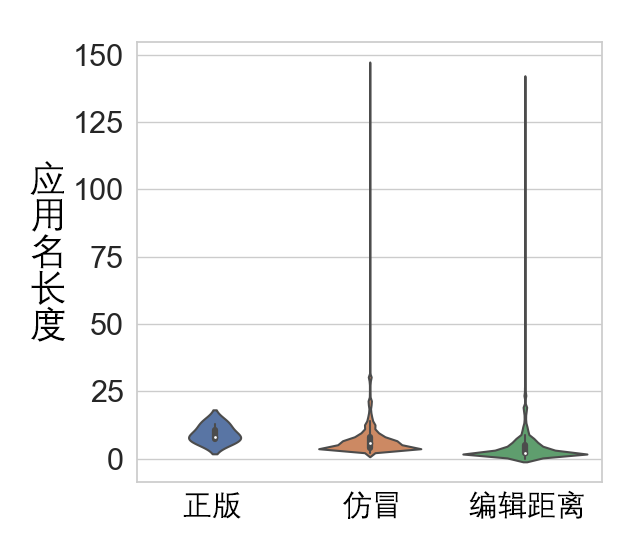
\includegraphics[width=0.333\textwidth]{./Figures/edwin-RQ1-2(a).png}}\hfill
    \subfloat[包名\label{fig:pkgname}]{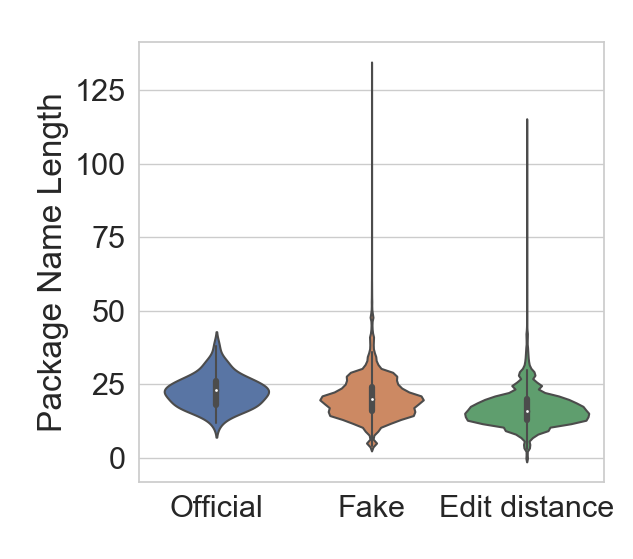
\includegraphics[width=0.333\textwidth]{./Figures/edwin-RQ1-2(b).png}}\hfill
    \subfloat[样本大小\label{fig:size}]{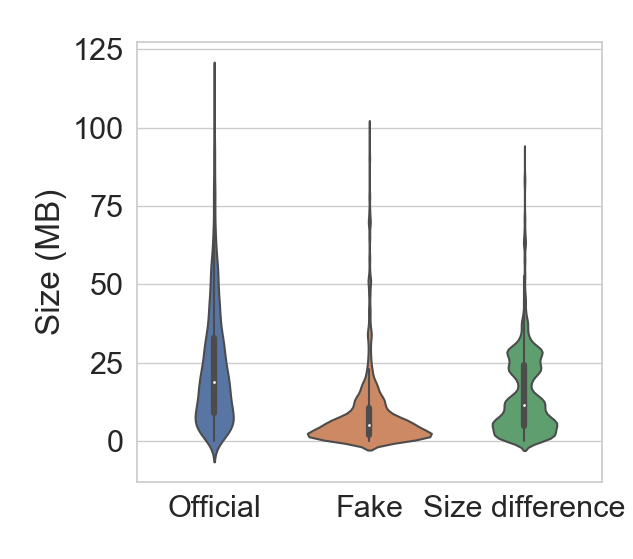
\includegraphics[width=0.333\textwidth]{./Figures/edwin-RQ1-2(c).png}}\hfill
	\caption{对App各项属性的统计结果}
	\label{fig:Statistic_fake_and_official}
	\vspace{-5mm}
\end{figure*}

% Fig.~\autoref{fig:Statistic_fake_and_official} is consist of three violin plots,\footnote{\url{https://en.wikipedia.org/wiki/Violin_plot/}} representing our statistics on app names, package names and package sizes, respectively.
\autoref{fig:Statistic_fake_and_official}由三个小提琴图\footnote{\url{https://en.wikipedia.org/wiki/Violin_plot}}组成,分别表示了本文在应用名、包名和APK包大小上的统计信息。
% In each ``violin'', the white dot represents the median, the thick bar in the middle represents the interquartile range while the thin bar represents 95\% confidence interval.
在每个``小提琴''中,中间的黑色粗条表示四分位数范围,粗条中间的小白点表示数据的中位数,而黑色细条表示95\%置信空间。

% Fig.~\autoref{fig:appname} shows the statistic information on app names of official samples, fake samples, and the edit distance between them.
\autoref{fig:appname}展示了分别在官方样本、仿冒样本的应用名和两者间编辑距离的统计数据。
% Both the white dot in ``Official'' violin and the one in ``Fake'' violin are at a similar level near the value ``6'', which means the average length of app names of both official samples and fake samples are close to each other.
其中``官方''图例和``仿冒''图例中的小白点都在接近数值``6''的位置,说明官方样本和仿冒样本的应用名的平均长度十分相近。
% The overall distribution of these two data groups have similar bodies, signals that they are also similar as well.
这两个数据组之间的数据分布的主体略微相近,也表面了他们的相似程度。
% What's more, the median value of edit distance is low (``2'' on $y$-axes), meaning that half of the fake apps get their names by modifying less than 3 characters from the corresponding official apps' names.
更重要的是,图中``编辑距离''图例的中位数值十分低(在$y$轴上为``2''的位置)。
这意味着过半数仿冒应用通过从官方App的应用名中修改少于3个字符来获得其应用名。
% This is a proof indicating that most fake apps are using a similar name to an official name.
这表示大部分仿冒应用正在使用与官方App非常相似的应用名。
% At the same time, we notice that some fake apps have pretty long names (there is one with a name of 146-character-long length).
与此同时,笔者也留意到了一些仿冒应用有着异乎寻常的长名称(其中最长的仿冒样本的应用名中甚至有146个字符)。
% Many of those outliers are samples uploaded by fake authors, maybe for testing purpose to explore the vetting mechanism.
% The other purpose is to associate users' search keywords as far as possible.
笔者认为这些异常样本有可能是出于测试市场审查机制的目的而被上传到市场上的。
另一种可能是,一些长应用名拼合了多个热门App的名称(比如``潮流女装-美丽说蘑菇街淘宝天猫京东美团精选''),这可能是为了应用更容易地被用户搜索到而采取的策略。

% Fig.~\autoref{fig:pkgname} shows the result on package names.
\autoref{fig:pkgname}显示了针对包名的结果。
% Like the plots in Fig.~\autoref{fig:appname}, the difference between the average length of package names of official apps and the average length of package names of fake apps is still tiny (they are of value ``23'' and ``20'', respectively).
和\autoref{fig:appname}类似,官方App的平均包名长度和仿冒样本的平均包名长度依然很类似(双方的值分别为``23''和``20'')。
% Nonetheless, the median of edit distance between them is explicitly higher (``16'' on $y$-axes), which means it takes averagely 16 times modification to turn a fake package name to an official package name and vice versa.
然而,他们之间编辑距离的中位数则比应用名编辑距离的中位数明显更高(在$y$轴上``16''的位置),这意味着将一个仿冒应用的包名转换为一个官方App的包名平均需要16次修改,反之亦然。
% Thus, we infer that fake apps tend to use self-defined package names.
也就是说,官方App的包名和仿冒应用的包名会相当不一样。可以据此推出仿冒应用更倾向于使用自定义的包名。

% Fig.~\autoref{fig:size} reports package size information.
\autoref{fig:size}显示了APK包大小的信息。
% To better represent the trend, we eliminated some outliers: samples that are larger than 150MB (851 in 69,614 official samples (about 1\%) and 447 in 52,638 fake samples (less than 1\%), most of which are from 游戏 category).
为了能更好地显示结果,笔者作图前从数据集中剔除了一些极端样本:他们是大于150MB的APK包,在所有69,614个官方App的样本中占851个(约为1\%),在52,638个仿冒样本中占447个(少于1\%)。
这些极端样本大部分来源于``游戏''类别下。
% The figure shows that the median number of fake samples' size is around 5MB, while half of the official apps have a size greater than 18MB, meaning that fake apps are more likely to be
图表显示,仿冒样本大小的中位数约为5MB,而约半数的正版App有着大于18MB的大小。
因此,仿冒应用更有可能:

% (1) developed by their owners but not originated from repackaging official apps,
1) 由仿冒开发者自行开发,而不是使用重打包技术制作,因为重打包之后的应用通常不会在大小上与原版有太大差距;

% (2) malicious apps, for malicious apps are usually in small sizes.
2) 是恶意应用,因为恶意应用除了恶意代码之外,通常没有太多其他内容。
\vspace{1mm}

% In short, Fig.~\autoref{fig:Statistic_fake_and_official} tells that fake apps
简而言之,\autoref{fig:Statistic_fake_and_official}说明了仿冒应用:

% (1) prefer to use a similar (or even same) name to an official app's name, but they have their own package names and
1) 更倾向于用一个与正版App相似(甚至是相同)的应用名,但会使用自定义的包名;

% (2) are usually of a small size.
2) 通常大小更小。
\vspace{1mm}

% To a large extent, we owe the first point to the incompleteness of the information the app store displays on apps.
在很大程度上,笔者认为产生第一点结论的原因是应用市场上提供的App信息的缺失和用户对Android App了解的缺乏。
% In most app stores, when users browse an app's detail page, they can only see the app's name, description, user comments and ratings which are positive for leading users to download that app.
如\autoref{fig:app_detail_page}所示,在应用市场上,当用户浏览App的详情页时,能看到应用名、下载量、应用描述、其他用户对应用的评论和评分等信息。
% However, technical information rarely appears.
但是,大部分应用详情页上并不会出现技术详情,比如应用包名。而普通用户也不会了解Android App中包名和应用名的区别和关联。
% In some app markets, users don't even know how large an apk file is.
个别应用市场(如\autoref{fig:xiaomi_detail}所示的小米应用市场)上,应用的某些信息甚至被折叠了起来,用户要点开折叠页才能发现一个App会有多大。
因此,不会被普通用户关注的包名自然可能会出现各种五花八门的情况,而一定会显示的应用名则是越接近正版App越容易诱导用户下载。

\begin{figure*}[t]
	\centering
    \subfloat[360应用市场\label{fig:360_detail}]{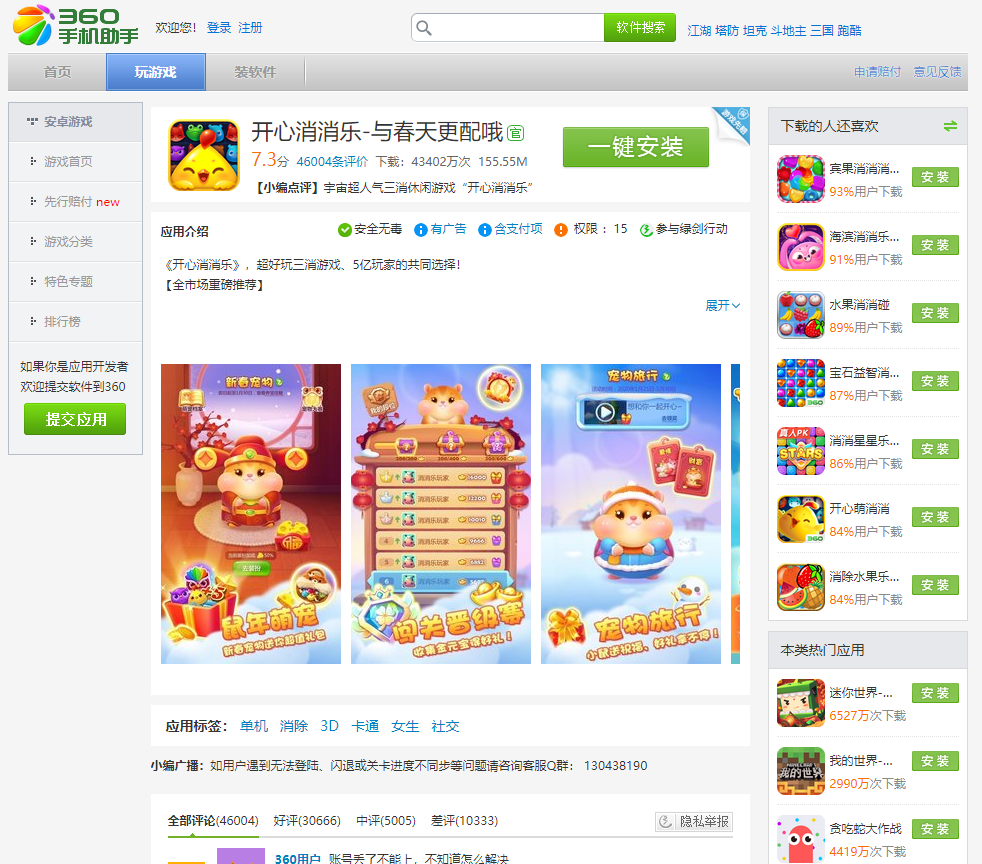
\includegraphics[width=0.49\textwidth]{./Figures/edwin-app-detail-360.png}}\hfill
    \subfloat[应用宝\label{fig:yyb_detail}]{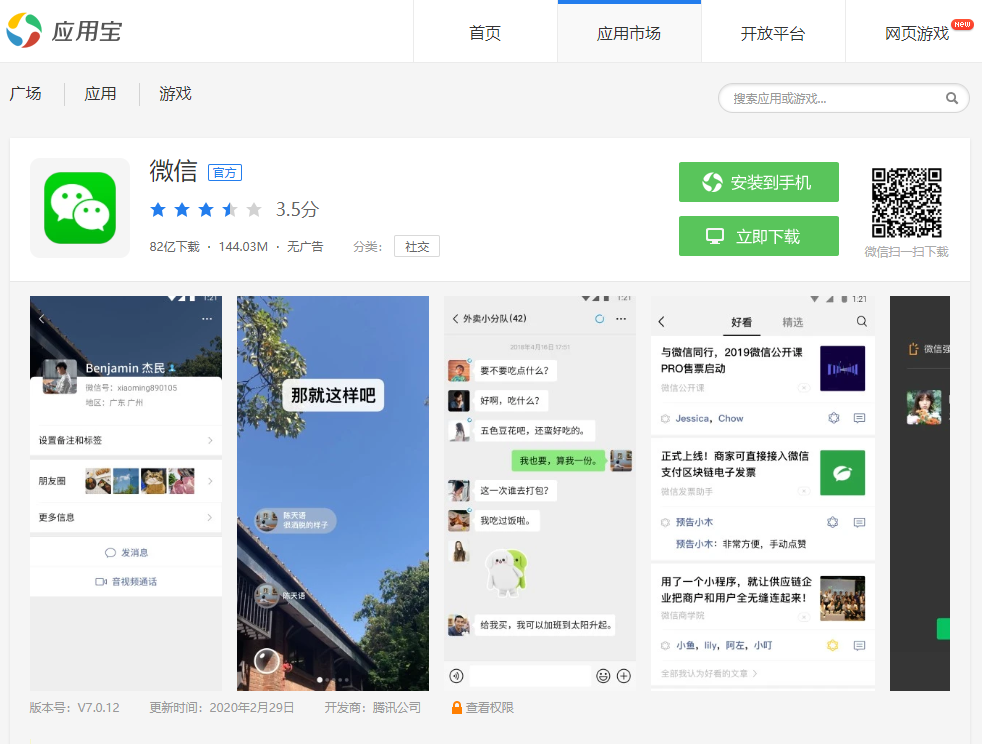
\includegraphics[width=0.49\textwidth]{./Figures/edwin-app-detail-yyb.png}}\hfill

	\subfloat[百度手机助手\label{fig:baidu_detail}]{
\includegraphics[width=0.49\textwidth]{./Figures/edwin-app-detail-baidu.png}}\hfill
    \subfloat[小米应用市场(部分信息被折叠)\label{fig:xiaomi_detail}]{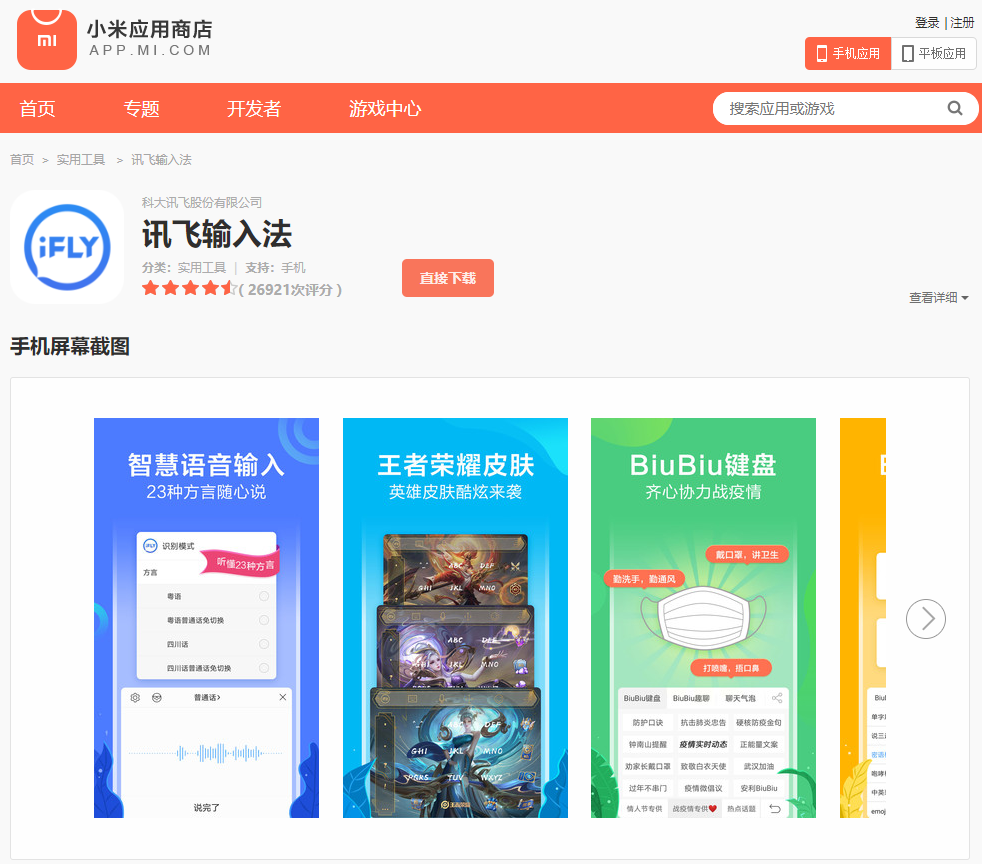
\includegraphics[width=0.49\textwidth]{./Figures/edwin-app-detail-xiaomi.png}}\hfill
	\caption{各大应用市场应用详情页(从桌面端浏览)}
	\label{fig:app_detail_page}
	\vspace{-5mm}
\end{figure*}
% \vspace{5mm}


% \noindent {\bf Case study 3.} \emph{Suspicious samples with official certificate}
\subsection{案例 1. 持有官方安全证书的可疑样本}

在人工浏览数据时,笔者发现了一个具有可疑应用名的样本---该样本声称自己是一个``破解版''的应用。
% Furthermore, we checked (1) if strange word (e.g., ``cracked") appears in our official samples' names, (2) whether or not an official app is signed by an official certificate from another developer, and (3) if one official sample has a suspicious package name.
于是,笔者针对所有69,614个持有官方证书的样本进行了以下几项筛选:
\begin{enumerate}
    \item 使用``破解''、``免费''等关键字搜索所有带正版证书的样本,筛选出带有可疑应用名的样本;
    \item 筛选所持安全证书与原开发者不一致的样本;
    \item 筛选出包名和同款App的多数样本不一致的样本。
\end{enumerate}

% Eventually we acquired 17 suspicious official samples, listed in table~\ref{table:suspicious_samples} are samples in each of these three kinds.
最终,本文获得了17个由正版开发者安全证书签署的可疑样本,其中三个样本的信息如\autoref{table:suspicious_samples}中所示,分别代表上述三项筛选得到的结果。
第一个名为\texttt{爱奇艺}的样本虽然由一个官方安全证书签名,但该安全证书和其他爱奇艺样本的却不一致。
对比之后,笔者发现该证书来自360手机助手,但360和爱奇艺并没有合作关系,因此这是个可疑的样本;
而第二个样本(\texttt{360手机助手})的可疑之处在于样本包名。多数\texttt{360手机助手}的包名为\emph{com.qihoo.appstore},也有少部分官方包名为\emph{com.qihoo.secstore},前者为\texttt{360手机助手}在国内第三方应用市场发行的应用包名,后者为Google Play官方应用市场上上架的包名。然而,其中一个使用了其官方安全证书签署的样本的包名却是\emph{com.kuyou.sdbgj.baidu},十分奇怪;
第三个样本则是在应用名中包含了``破解''字样。然而,正常的正版应用根本不会有这样的命名方式,所以笔者也认为这是一个可疑样本。
进行后续分析时,相关样本已被剔除出正版样本集合。

% \textsc{Virustotal} reports that only 2 of the 17 samples are benign, 2 are PUP and the other 13 samples are all malicious.
\textsc{Virustotal} 的检查结果显示,17个可疑样本中,只有2个是良性应用,2个是PUP,余下13个样本都被判定具有恶意行为。

\begin{table*}[htbp]
    \renewcommand{\arraystretch}{1}
    \small
    \centering
  \setlength{\belowcaptionskip}{-10pt}
    \caption{持有官方安全证书的可疑样本}
    \begin{tabular}{l l c c c c c c}
        \toprule
        {\bf 样本应用名} & {\bf 样本SHA1码} & {\bf 可疑之处} \\
        \midrule
        % 爱奇艺 & b86c55a509e8293b24138b166e9ff410f39e84b5 & 可疑证书(360手机助手) \\
        爱奇艺 & b86c55a509e8293b24138b166e9ff410f39e84b5 & 可疑证书\\
        % 360手机助手 & 2bb43c53b86d204d0040a8af6cb2a09cf9e93bb7 & 可疑包名(com.kuyou.sdbgj.baidu) \\
        \rowcolor{gray!15} 360手机助手 & 2bb43c53b86d204d0040a8af6cb2a09cf9e93bb7 & 可疑包名\\
        % Youku XL 破解版 & b55b7ef189d649aeb03443c5d1ab57c9031d624e & 可疑应用名(``破解版") \\
        Youku XL 破解版 & b55b7ef189d649aeb03443c5d1ab57c9031d624e & 可疑应用名 \\
        \bottomrule
    \end{tabular}
    \label{table:suspicious_samples}
\end{table*}

% Despite the possibility that these certificates were somehow leaked to the underground industry, it is more likely that some attackers penetrated the protection scheme.
鉴于这17个样本都是持有官方安全证书签名的,笔者起初不禁怀疑是否有应用厂家不慎泄露了自己的安全密钥库,从而导致了这些样本的出现。
然而,如果真的是因为厂家泄露密钥库,一来很有可能会导致恶意开发者使用官方安全证书大量生产恶意应用,二来对应厂家也会出于安全考虑马上更换新的包名和安全证书。
本研究的数据并不支持以上猜想带来的两点结果,所以本文不认为这是由于安全证书泄露导致了这些可疑样本的产生。

除去这个可能性,本文认为更有可能的原因是某些仿冒应用开发者掌握了穿透/绕过Android系统签名机制的技术,从而产生了这些样本。

% As far back as December 2017, Google had confirmed and revealed a backdoor on V1 signature scheme (CVE-2017-13156)~\cite{android_security_bulletin}, by which hackers can inject any content into an apk at will without modifying its certificate information.
时间回溯到2017年12月,Google确认并公布了V1版本应用签名机制的一个后门(CVE-2017-13156)~\cite{android_security_bulletin}。
通过这个后门,黑客可以在不修改APK包安全证书信息的情况下,向APK包里注入任意内容。
% An alternative solution, V2 signature scheme, has been launched at least one year before that.
而早在这个漏洞被公布的至少一年之前,Google就已经发布了作为V1版签名机制的替代解决方案,也就是V2版应用签名机制。
% In order to confirm if these apps are using the risky V1 scheme, we used a tool, apksigner, provided by Google to verify which signature schemes these samples are using.
这看起来十分有可能是导致这些可以样本产生的原因,某些恶意开发者利用了V1版本签名机制的漏洞,修改了APK包的基本信息。
为了确认这些样本是否采用了具有风险的V1版应用签名机制,本文使用了apksigner来检测这些样本使用的签名机制版本。
apksigner是Google官方提供的一个命令行工具,它被集成在Android SDK中,既是APK包编译打包过程中为APK包进行数字签名的工具,也可以用来验证APK包使用的签名机制版本,又或者是验证APK的签名是否有效。

% It ends up that all 17 samples are using V1 signature scheme.
apksigner的结果显示,所有17个样本都只使用了V1版本的应用签名机制。
% With actually knowing that V1 is no longer safe, developers still refuse to embrace the safer scheme, which is really disappointing.
在了解到V1版本签名机制已经不再安全的情况下,仍有部分开发者由于各种原因没有接受更新也更安全的签名方案,这个结果有点令人失望。

\noindent\fbox{
	\parbox{0.95\linewidth}{
		% \textbf{Remark 1}: Most certificates link with only a number of fake apps, which is highly possible to be a fake developers' evasive strategy.
		\textbf{本节小结}: 绝大部分安全证书只与少数仿冒样本有所关联。这很可能是仿冒开发者规避市场监管机制采用的策略。
		% Moreover, we observe that fake apps do tend to use official app names or names alike.
		同时,本文也观测到仿冒应用倾向于于官方App相同或者是十分相似的应用名。
		% Nonetheless, fake apps and official apps are not resemble in terms of package names or apk sizes, disclosing that repackaged apps are not mainstream in fake apps.
		但是,仿冒样本和官方App在包名和APK包大小方面都不相似,这表明重打包应用在仿冒应用中并不普遍存在。
        最后,如果良性应用的开发者不遵从最新的安全标准发布应用,可能会导致十分严重的安全问题。
	}
}



% \subsection{Quantitative Study on Fake Samples}
\section{影响仿冒应用数量的因素}
\label{sec:quantitativeStudy}
% It is valid to assume that fake app developers are driven by profits, hence there is a likelihood that the number of fake app is correlated to their source market, popularity and categories.
天下熙熙,皆为利来;天下攘攘,皆为利往。
不妨假设获利是驱动仿冒应用开发者的最终目标,进而假设仿冒应用的数目与其来源市场、受欢迎程度及其应用分类密切相关。
因为一个应用越受欢迎,就越可能获利,对仿冒应用也是如此。
% In addition, the update frequency can be taken in as a factor, too.
此外,App的更新频率也可以被视作一个潜在因素,频繁更新的App或许会阻碍仿冒应用开发者对其进行仿冒。

\subsection{仿冒应用的来源}

本研究中搜集的应用样本来源于多个不同的应用市场,每个市场架上的应用数量不一,其审核、监管力度也并不一致。
因此笔者不禁好奇,应用商店架上的应用样本数量是否会跟仿冒应用的数量有关系?
为此,本节有了以下假设:

% \noindent{\bf Hypo 2.1:} {The rate of fake samples is related to the number of apps a market contains.}
{\bf 假设 2.1}:仿冒样本的比率与应用市场架上的App数量有关联。

% Correspondingly, we define our research questions as follows:
与之相对,本节有研究问题如下:

% \noindent{\bf RQ 2.1}: Where are these fake samples mainly from?
{\bf RQ 2.1}:这些仿冒应用市场都集中来源于哪里?哪个应用市场有最多的仿冒应用?

根据各个样本的来源,本节从数据统计角度分析了结果。

% \noindent{\bf Answer to RQ 2.1.} Fig.~\autoref{fig:Sample_source} shows the samples' origin.
{\bf RQ 2.1. 结果} \autoref{fig:Sample_source} 展示了本研究收集到的所有样本的来源。
% From the left subplot, \texttt{Baidu App Store} not only provides the largest sample number among all 31 different app sources, but is also the source where most fake samples are from.
左图显示,在本研究收集数据的所有31个应用商店中,源于\texttt{百度手机助手}的样本量是最大的。
同时,从\texttt{百度手机助手}中搜集到的仿冒样本也是最多的。
% Fake sample rates are displayed on the right subplot.
各个应用市场的仿冒率在右图呈现。

\begin{figure*}[htbp]
	\centering
  \setlength{\belowcaptionskip}{-10pt}
	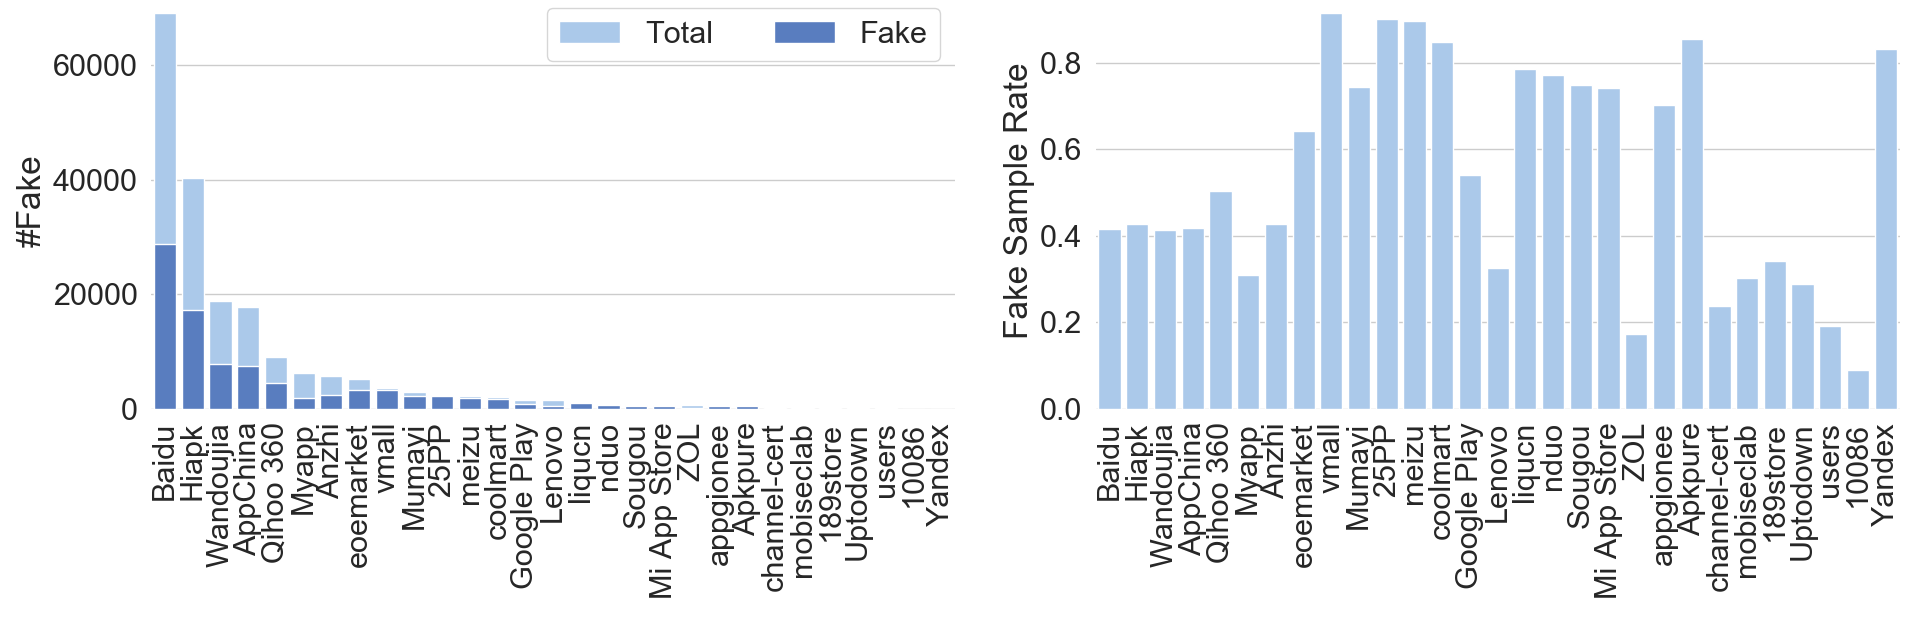
\includegraphics[width=\textwidth]{./Figures/edwin-Number_of_samples_collected_markets_3.png}
	\caption{从不同应用市场中收集到的应用数量以及各市场仿冒率}
	\label{fig:Sample_source}
\end{figure*}

\begin{Def}
    仿冒率

    某款App~$a$的仿冒率$fake~sample~rate_a$指与其关联的仿冒样本的数量$fake_a$与该App正版样本的数量$total_a$的商(\autoref{equ:fake_rate_app})。

    某应用市场$AS$的仿冒率$fake~sample~rate_{AS}$则是其中包含的所有目标App的均值(\autoref{equ:fake_rate_mkt})。
\end{Def}

\begin{equation}
    fake~sample~rate_a = \frac{fake_a}{total_a}
    \label{equ:fake_rate_app}
\end{equation}
\begin{equation}
    fake~sample~rate_{AS} = Avg(fake~sample~rate_a, \forall a \in \text{\{目标App\}})
    \label{equ:fake_rate_mkt}
\end{equation}
\vspace{0.5mm}

% Although both \texttt{Baidu App Store}~\cite{Baiduappstore} and \texttt{Hiapk}~\cite{Hiapk} hold a fake sample rate of about 40\%, the number of fake samples from \texttt{Baidu App Store} exceeds \texttt{Hiapk} to a great extent due to its dominant total sample number.
尽管\texttt{百度手机助手}~\cite{Baiduappstore}和\texttt{安卓市场}~\cite{Hiapk}的仿冒率均为40\%左右,在所有的31个渠道中处于中等水平,但由于源于这两个渠道的样本基数最大,所以从这两个应用市场搜集到的仿冒样本数也是最多的。

% Although no connection between the number of fake samples and market can be found from our data, we notice that the relationship between apps and markets may affect the fake rate.
图中数据显示,应用市场的样本数量和仿冒率并没有直接联系,但是本节仍然有一个有趣的发现,那就是App本身和市场的关系有可能是影响App仿冒率的一个因素。
% This is well supported by the low fake rate of \texttt{Myapp}~\cite{Myapp} -- the app market provided by \texttt{Tencent}, which is also the 12 out of 50 developers in our target apps.
\texttt{腾讯}旗下的应用市场\texttt{应用宝}~\cite{Myapp}中较低的仿冒率可以很好地为这个发现提供数据支持,因为本研究的50款目标App中,有12款都是腾讯公司开发的应用。

\subsection{其他因素对仿冒样本数量的影响}
% Accordingly, we hypothesize the following factors may influence the number of fake samples of an app:
除了市场本身之外,本节还假设以下这些因素可能会影响某款App对应的仿冒样本数量:

% \noindent{\bf Hypo 2.2:} The number of fake apps are closely related to how popular an app is.
{\bf 假设 2.2}:仿冒应用的数量与其对应的正版App的受欢迎程度有密切联系。

% \noindent{\bf Hypo 2.3:} Update frequency effects the number of fake samples.
{\bf 假设 2.3}:应用的更新频率影响着其对应仿冒应用的数量。

% \noindent{\bf Hypo 2.4:} Category is a factor influencing the fake sample number.
{\bf 假设 2.4}:App类别是影响仿冒应用数量的因素之一。

与三个假设对应的是三个研究问题:

% \noindent{\bf RQ 2.2}: Does the popularity of an app affect the number of its fake samples?
{\bf RQ 2.2}:一个App受欢迎的程度会影响对其仿冒的应用数量吗?

% \noindent{\bf RQ 2.3}: Does an app's update frequency influence its fake sample's number?
{\bf RQ 2.3}:一个App的更新频率会影响对其仿冒的应用数量吗?

% \noindent{\bf RQ 2.4}: Is the number of fake samples related to the app's category?
{\bf RQ 2.4}:一个App所在类别会影响对其仿冒的应用数量吗?

对于这三个研究问题,本节使用了皮尔逊积矩相关系数(Pearson product-moment correlation coefficient,简称PPMCC)来衡量应用数量和问题对应的几个维度的关联性。

% \noindent{\bf Answer to RQ 2.2.}
{\bf RQ 2.2. 结果}
% Intuitively, the more popular an app is, the more possible it would get shammed, for fake developers would mislead users to download their apps to gain profits.
从直觉上看,某款App越受欢迎,仿冒应用开发者就越有动机对其仿冒,然后诱导用户下载仿冒版本以获取利润。

% Note that each app has different amount of samples (including official samples and fake samples), processing our measurement directly based on the number of fake samples is incorrect.
要注意的是,每款目标App都有不同的样本数(无论是官方的或是仿冒的),所以在这里不能拿仿冒样本的数量直接作比较。
% To counteract this bias, each fake count should be regularize into a \textit{fake sample rate}, the rate of fake samples in all collected samples of an app.
为了消除偏差,本文将样本数量归一化,使用\autoref{equ:fake_rate_app}定义的仿冒率对每个目标App进行比较。
% Next, we employ a metric called \textit{Pearson product-moment correlation coefficient (PPMCC)} to reveal relativeness between an app's fake sample number and its popularity, which uses the regularized fake sample rates and monthly activeness indicators (MAI) obtained from Analysys~\cite{yiguanqianfan}.
接下来,本文使用了皮尔逊积矩相关系数来计算一款App被仿冒的严重程度与其热度是否具有相关性。
相关计算会使用上述的仿冒率和从易观千帆~\cite{yiguanqianfan}获取的App月度热度指数计算。

\begin{Def}
    皮尔逊积矩相关系数

    两个变量之间的皮尔逊相关系数定义为两个变量之间的协方差和标准差的商(\autoref{equ:PPMCC})。
\end{Def}
\begin{equation}
    p_x,_y = corr(X,Y)=\frac{cov(X,Y)}{\sigma_x\sigma_y}=\frac{E[(X-u_x)(Y-u_y)]}{\sigma_x\sigma_y}
    \label{equ:PPMCC}
\end{equation}
\vspace{0.5mm}

% This value ranges from -1 to 1, the closer the PPMCC value is to 0, the weaker correlation between the two factors is indicated.
\autoref{equ:PPMCC}的值域为$[-1, 1]$,该值越接近0,表示两个变量之间的相关关系越弱。
% Surprisingly, according to our data, the value of PPMCC between this two factors is 0.246, revealing that the fake sample number and an app's popularity only hold their relativeness on a weak level, which does not match our expectation.
出乎笔者意料的是,数据显示,两个因子之间的相关系数只有0.246。
这表明仿冒应用的数量和App的热度在相关性上只处于较弱水平,和笔者的预期并不符合。

% \noindent{\bf Answer to RQ 2.3.}
{\bf RQ 2.3. 结果}
% We assume the update frequency is related to the number of fake samples of an app, for updates can usually help keep a software from being attack.
笔者猜想更新频率有可能会与App被仿冒的次数相关联,因为升级通常会有漏洞修复等举措,可以帮助App免受攻击。
% The higher the update frequency is, the safer an app is supposed to be.
所以一款App的更新频率越高,其安全性能应该就会越好。

% To estimate the average update frequency of our target apps, the time when an app's official sample was crawled and when its latest official samples were crawled is marked.
为了评估一款目标App的平均更新频率,笔者标记了每个官方应用样本被发行时的时间,精确到日。
% The difference between them is then divided by the number of that app's existing version to obtain an update frequency, with unit day/version.
然后,再找到最新发布的那个样本和最早发布的那个样本,求出他们发行时间的差值的绝对值与版本数的商,即为平均更新频率(单位:天/版本)

% The result PPMCC value of 0.084 shows that the connection between an app's update frequency and its fake sample rate barely exists.
相关系数的计算结果表示,更新频率和仿冒数量之间的关联度只有0.084,意味着两者之间几乎没有关联。
% We attribute this result to two reasons:
笔者认为这个结果由两个原因导致:

% (1) The high update frequency (10 days/version on average for apps in our dataset) indicates app developers may not fix security issues in per update, weakening the function of update frequency as a security indicator.
1)在本研究的数据集中,每款App的平均更新间隔为10天/版本。
这个较高的更新频率表面开发者可能不会每次都在更新中修正安全性问题,从而削弱了更新频率作为安全性指标的功能。

% (2) A large portion of fake samples in our dataset are not derived from repackaging. To this end, fake developers can produce fakes regardless of how well the official apps are protected.
2)结合前文的结果,数据集中的大部分仿冒样本都不是重打包应用,而是仿冒应用开发者自行开发的。
因此,无论官方版本受到的保护程度如何,仿冒应用开发者都可以制造出对应的仿冒应用。

% \noindent{\bf Answer to RQ 2.4.}
{\bf RQ 2.4. 结果}
% Some categories are potentially more profitable than others.
某些App类别比其他类别更有可能带来收益。
% A report from the app marketing company LIFTOFF~\cite{LIFTOFF_report} forecasts gaming to be the next most billable area.
根据一份来自App营销机构LIFTOFF~\cite{LIFTOFF_report}的报告预测,在未来,\texttt{游戏}类有望成为带来最高收入的应用分类。

\begin{ThreePartTable}
\centering
\renewcommand{\arraystretch}{1.05}
\footnotesize
\setlength{\belowcaptionskip}{-5pt}
\vspace{1mm}
% \rowcolors{2}{gray!15}{white}
\begin{longtable}{l l c c c c c c}
\caption{目标App与其相关统计}\label{table:data-statistics}\\
\toprule
{\bf 应用名} & {\bf 类别} & \begin{tabular}[c]{@{}c@{}}{\bf 月度热} \\ {\bf 度指数} \end{tabular} & \begin{tabular}[c]{@{}c@{}}{\bf 更新频率} \\ {\bf (天/版本)} \end{tabular} & {\bf 样本总数} & \begin{tabular}[c]{@{}c@{}}{\bf 仿冒} \\ {\bf 样本数} \end{tabular} & {\bf 仿冒率} & \begin{tabular}[c]{@{}c@{}}{\bf 平均仿} \\ {\bf 冒延迟} \end{tabular} \\
\midrule
{\bf 微信}\tnote{*} & {\bf 社交网络} & {\bf 91.2K} & {\bf 6.4} & {\bf 9248} & {\bf 6447} & {\bf 69.7\%} & {\bf 12.1} \\
\rowcolor{gray!15} {\bf QQ}\tnote{*} & {\bf 社交网络} & {\bf 54.6K} & {\bf 10.7} & {\bf 11167} & {\bf 3780} & {\bf 33.8\%} & {\bf 9.2} \\
爱奇艺 & 视频 & 53.5K & 6.4 & 7586 & 3481 & 45.9\% & 9.3 \\
\rowcolor{gray!15} 支付宝 & 生活 & 48.1K & 10.2 & 983 & 231 & 23.5\% & 10.1 \\
{\bf 淘宝}\tnote{*} & {\bf 移动购物} & {\bf 47.5K} & {\bf 7.0} & {\bf 6003} & {\bf 3010} & {\bf 50.1\%} & {\bf 8.1} \\
\rowcolor{gray!15} 腾讯视频 & 视频 & 47.3K & 6.3 & 1429 & 68 & 4.8\% & 10.7 \\
优酷 & 视频 & 40.9K & 7.3 & 2058 & 262 & 12.7\% & 6.7 \\
{\bf 新浪微博}\tnote{*} & {\bf 社交网络} & {\bf 39.2K} & {\bf 5.3} & {\bf 5947} & {\bf 2715} & {\bf 45.7\%} & {\bf 5.7} \\
\rowcolor{gray!15} WiFi万能钥匙 & 系统工具 & 36.4K & 3.1 & 4808 & 2999 & 62.4\% & 3.0 \\
搜狗输入法 & 系统工具 & 33.3K & 11.0 & 898 & 40 & 4.5\% & 21.8 \\
\rowcolor{gray!15} 百度 & 资讯 & 32.4K & 11.1 & 15651 & 3514 & 22.5\% & 12.8 \\
腾讯新闻 & 资讯 & 28.7K & 8.5 & 1051 & 11 & 1.0\% & 8.9 \\
\rowcolor{gray!15} QQ浏览器 & 资讯 & 27.8K & 5.6 & 1369 & 43 & 3.1\% & 11.6 \\
今日头条 & 资讯 & 27.4K & 4.4 & 3538 & 179 & 5.1\% & 5.6 \\
\rowcolor{gray!15} 应用宝 & 应用市场 & 27K & 11.4 & 2419 & 266 & 11.0\% & 11.6 \\
快手 & 视频 & 24.4K & 3.2 & 8273 & 4270 & 51.6\% & 3.5 \\
\rowcolor{gray!15} 腾讯手机管家 & 系统工具 & 24.2K & 8.7 & 2463 & 1340 & 54.4\% & 8.7 \\
高德地图 & 生活 & 24K & 6.5 & 1225 & 51 & 4.2\% & 13.1 \\
\rowcolor{gray!15} 酷狗音乐 & 音乐 & 23K & 8.6 & 1313 & 122 & 9.3\% & 12.2 \\
QQ音乐 & 音乐 & 21.7K & 9.4 & 1132 & 65 & 5.7\% & 14.6 \\
\rowcolor{gray!15} 百度地图 & 生活 & 21.3K & 8.8 & 2609 & 1438 & 55.1\% & 15.3 \\
抖音 & 视频 & 19.4K & 11.1 & 317 & 12 & 3.8\% & 8.3 \\
\rowcolor{gray!15} {\bf 京东}\tnote{*} & {\bf 移动购物} & {\bf 18.5K} & {\bf 10.9} & {\bf 5000} & {\bf 2377} & {\bf 47.5\%} & {\bf 12.3} \\
UC浏览器 & 资讯 & 16.7K & 7.4 & 4232 & 1624 & 38.4\% & 7.0 \\
\rowcolor{gray!15} 360手机卫士 & 系统工具 & 15.4K & 12.4 & 3670 & 1423 & 38.8\% & 19.1 \\
全民K歌 & 音乐 & 14.7K & 21.1 & 618 & 215 & 34.8\% & 17.3 \\
\rowcolor{gray!15} 美团 & 生活 & 13K & 8.0 & 4752 & 1415 & 29.8\% & 6.9 \\
{\bf 拼多多}\tnote{*} & {\bf 移动购物} & {\bf 12.9K} & {\bf 6.6} & {\bf 2327} & {\bf 551} & {\bf 23.7\%} & {\bf 7.8} \\
\rowcolor{gray!15} {\bf 王者荣耀}\tnote{*} & {\bf 游戏} & {\bf 12.5K} & {\bf 15.5} & {\bf 2350} & {\bf 1319} & {\bf 56.1\%} & {\bf 12.3} \\
美图秀秀 & 摄影录像 & 12.4K & 5.4 & 1705 & 784 & 46.0\% & 5.8 \\
\rowcolor{gray!15} 火山小视频 & 视频 & 12.2K & 11.9 & 410 & 16 & 3.9\% & 9.6 \\
墨迹天气 & 生活 & 12K & 4.2 & 10081 & 7093 & 70.4\% & 4.7 \\
\rowcolor{gray!15} 滴滴出行 & 生活 & 11.8K & 8.6 & 943 & 117 & 12.4\% & 7.0 \\
华为应用市场 & 应用市场 & 11.8K & N/A & 0 & 0 & 0.0\% & N/A\\
\rowcolor{gray!15} {\bf 开心消消乐}\tnote{*} & {\bf 游戏} & {\bf 11.2K} & {\bf 19.7} & {\bf 2406} & {\bf 1738} & {\bf 72.2\%} & {\bf 20.6} \\
酷我音乐盒 & 音乐 & 11K & 2.9 & 3778 & 69 & 1.8\% & 4.2 \\
\rowcolor{gray!15} 西瓜视频 & 视频 & 11K & 11.5 & 866 & 100 & 11.5\% & 8.8 \\
OPPO应用商店 & 应用市场 & 10.8K & N/A & 0 & 0 & 0.0\% & N/A\\
\rowcolor{gray!15} 猎豹清理大师 & 系统工具 & 9.9K & 10.3 & 1803 & 388 & 21.5\% & 13.5 \\
360清理大师 & 系统工具 & 9.6K & 17.3 & 327 & 8 & 2.4\% & 8.5 \\
\rowcolor{gray!15} 360手机助手 & 应用市场 & 9.2K & 7.6 & 1616 & 137 & 8.5\% & 8.4 \\
WiFi管家 & 系统工具 & 8.8K & 19.5 & 1636 & 658 & 40.2\% & 15.7 \\
\rowcolor{gray!15} 讯飞输入法 & 系统工具 & 8.6K & 6.0 & 1451 & 8 & 0.6\% & 10.1 \\
百度手机助手 & 应用市场 & 8.2K & 11.4 & 3849 & 437 & 11.4\% & 14.5 \\
\rowcolor{gray!15} 小米应用市场 & 应用市场 & 7.8K & N/A & 0 & 0 & 0.0\% & N/A\\
{\bf WPS Office}\tnote{*} & {\bf 商务办公} & {\bf 7.4K} & {\bf 6.0} & {\bf 1152} & {\bf 69} & {\bf 6.0\%} & {\bf 7.8} \\
\rowcolor{gray!15} 美颜相机 & 摄影录像 & 7.1K & 5.3 & 1600 & 691 & 43.2\% & 6.3 \\
网易云音乐 & 音乐 & 7K & 10.5 & 616 & 6 & 1.0\% & 12.2 \\
\rowcolor{gray!15} 网易新闻 & 资讯 & 6.7K & 7.0 & 1441 & 93 & 6.5\% & 5.0 \\
{\bf QQ邮箱}\tnote{*} & {\bf 商务办公} & {\bf 6.6K} & {\bf 16.4} & {\bf 520} & {\bf 11} & {\bf 2.1\%} & {\bf 10.4} \\
\bottomrule
\end{longtable}
\vspace{-4mm}
\begin{tablenotes}
  % \item[*] Detailed descriptions are given in {\bf Answer to RQ 2.4}
  \item[*] 详情会在{\bf RQ 2.4. 结果}中给出
\end{tablenotes}
\end{ThreePartTable}

% Our 50 target apps are divided into 11 categories according to their functionalities, Table~\autoref{table:data-statistics} shows these categories and their corresponding fake sample rate.
根据应用功能划分,本研究的50款目标App可以被分为11个类别。
\autoref{table:data-statistics}按每款App的热度排序,展示了每款App的类别和他们的仿冒率,同时还有他们的更新频率、关联样本总数等数据。
% In the same category, the difference between apps on fake rate lies in an acceptable range.
在相同的类别下,多数应用之间的仿冒率差值都位置在一个合适的水平。
% Without doubt, entertainment related categories like \texttt{游戏} and \texttt{Social Network} attract more fake samples.
毫无疑问地,娱乐方向的类别(比如\texttt{游戏}和\texttt{社交网络})吸引了更多仿冒应用开发者对其仿冒。
% Another field, \texttt{Online shopping}, has also gained special love from fake developers because online shopping is rapidly developing in China.
而另一个类别\texttt{移动购物}也特别受到了仿冒应用开发者的``关照'',因为移动购物在中国也正在快速地发展。
% Relatively, \texttt{商务办公} is not that attractive to fake developers, the average fake sample rate of this filed is only 4.05\%.
相对来说,商务方向的\texttt{商务办公}分类的应用就不是那么地吸引仿冒应用开发者了,这个领域下的App平均仿冒率只有4.05\%。
% Apps in these four categories are marked in bold in the table.
上述四个类别的应用都在表中被加粗标识,读者可以自行查阅。

% The result matches the observation in our daily life, people always tend to use mobile devices for entertainment instead of business purpose.
这个结果与笔者在日常生活中观察到的结果相符,比起商务类用途,普罗大众更倾向于使用移动设备用作娱乐用途,消遣时间。
% It's pretty interesting to discover that the number of fake samples in a way reflects how people use their phone in their daily lives.
仿冒应用的数量从某种角度上反映了人们在日常生活中如何使用移动设备,这是个十分有趣的发现。

% \noindent{\bf Case study 2.} \emph{Fake samples in different gaming apps}
\subsection{案例 2. 游戏类别下的仿冒应用}

% Gaming apps in our target app list (i.e. \texttt{\small ArenaofValor} and \texttt{\small HappyElements}) attract a number of fake samples.
正如\autoref{table:data-statistics}中数据所示,\texttt{游戏}类应用(\texttt{王者荣耀}和\texttt{开心消消乐})吸引了大批的仿冒应用样本。
% To figure out what do these samples look like, we randomly downloaded some of the fake samples of the 2 gaming apps (7 samples for each) and installed them on our testing device.
出于性能考虑,此处的数据中只提取了APK包的基本信息,并没有对收集到的每个APK文件进行详细的分析。
因此,为了弄清楚这些仿冒应用究竟是怎么样的,笔者随机从这两款游戏App的仿冒样本中选择了一些样本(每款应用选择7个仿冒样本),然后将这些样本安装到了实验设备上。

% Fig.~\ref{fig:screenshot_all} shows how these samples look like on a real Android phone, official apps are marked with green frames.
\autoref{fig:screenshot_all}展示了这些样本在真实的Android设备上安装之后的实际外观。
官方渠道下载的正版App在图片中由绿色边框标记出。
% Apparently, fake samples have either a similar name or a similar icon to official ones.
明显地,与官方应用相比,仿冒应用或者有一个和官方应用名十分相似的应用名,或者在图标上和官方相近甚至相同。

\begin{figure}[htbp]
    \centering
    \subfloat[两种游戏App与其仿冒\label{fig:screenshot_all}]{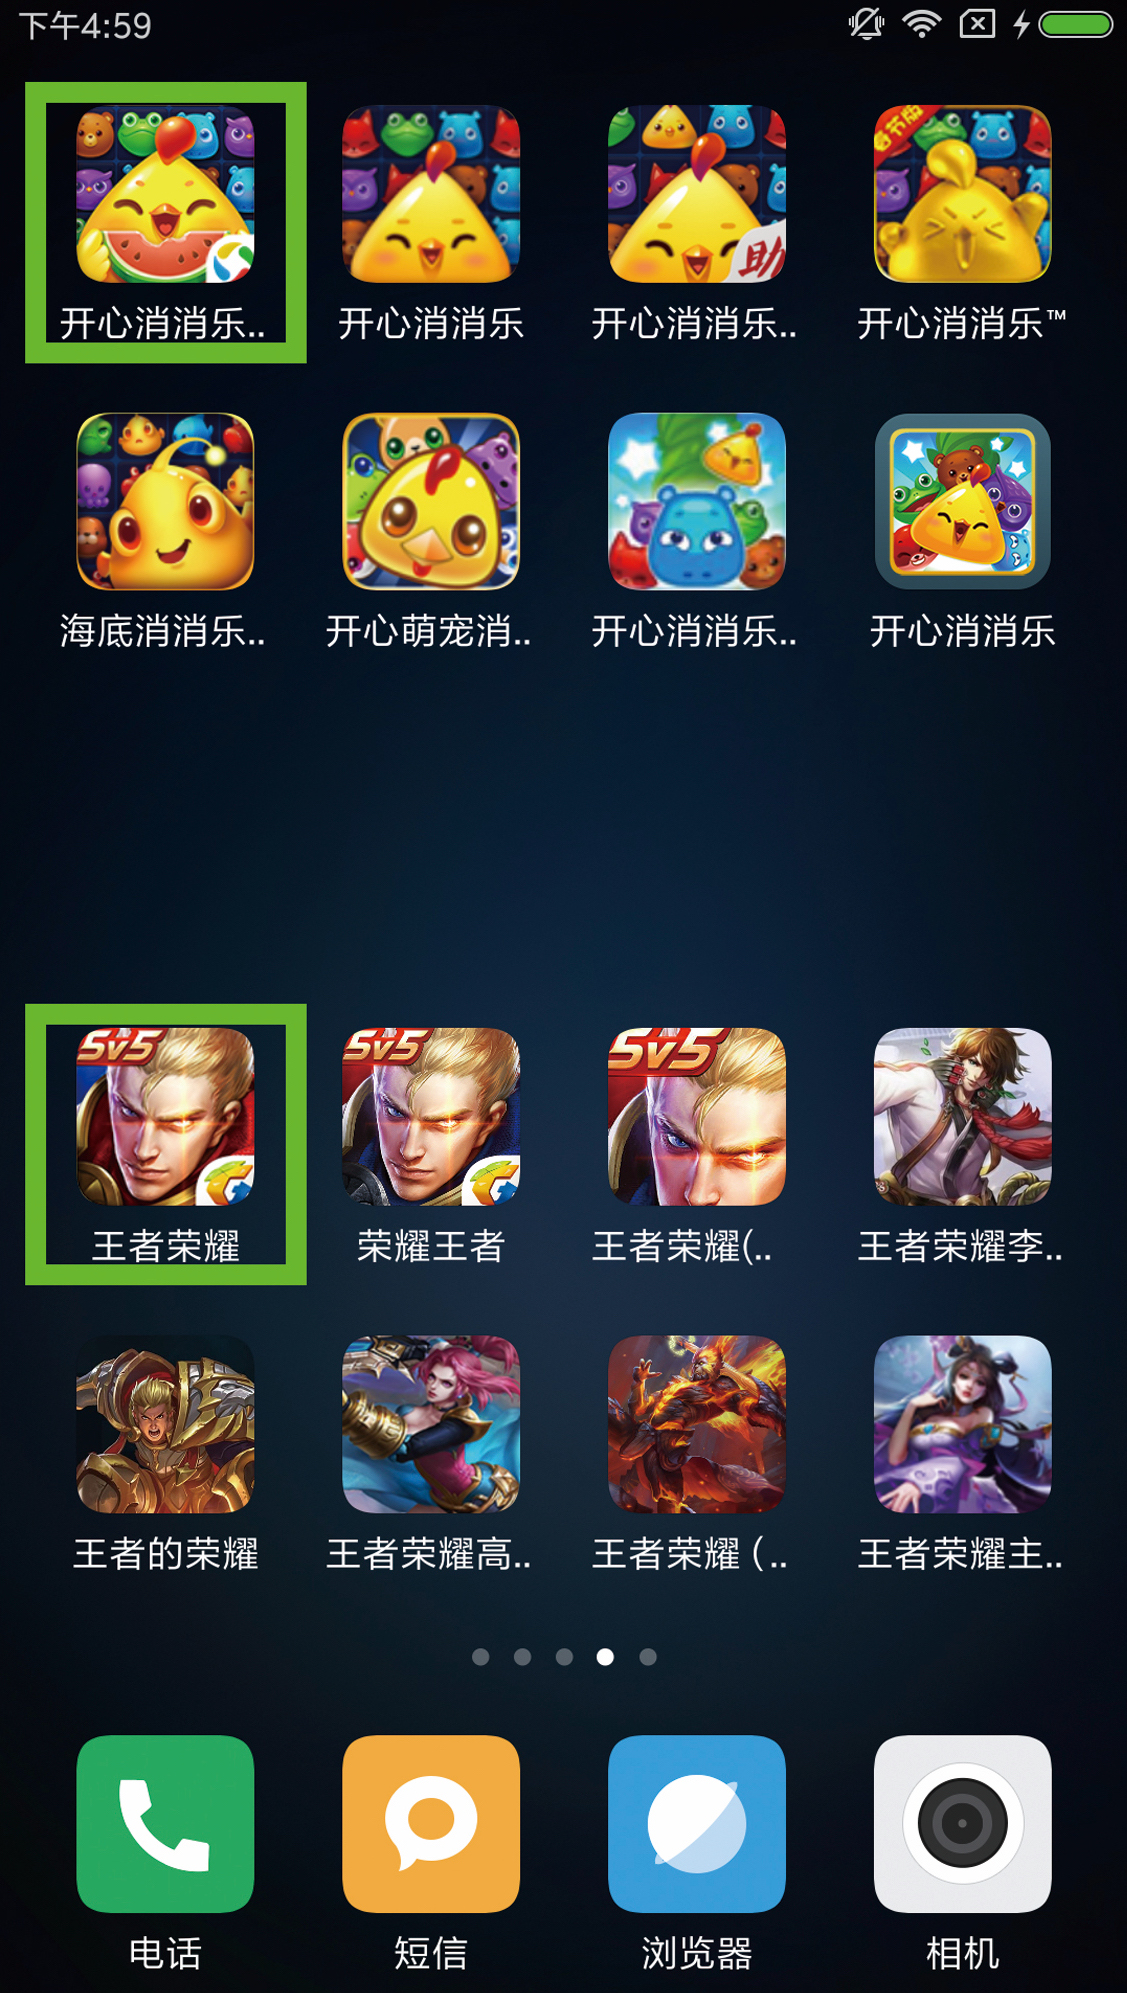
\includegraphics[width=0.3\textwidth]{./Figures/edwin-screenshot1.jpg}}\hfill
    \subfloat[正版\textit{\small 开心消消乐}\label{fig:screenshot_official}]{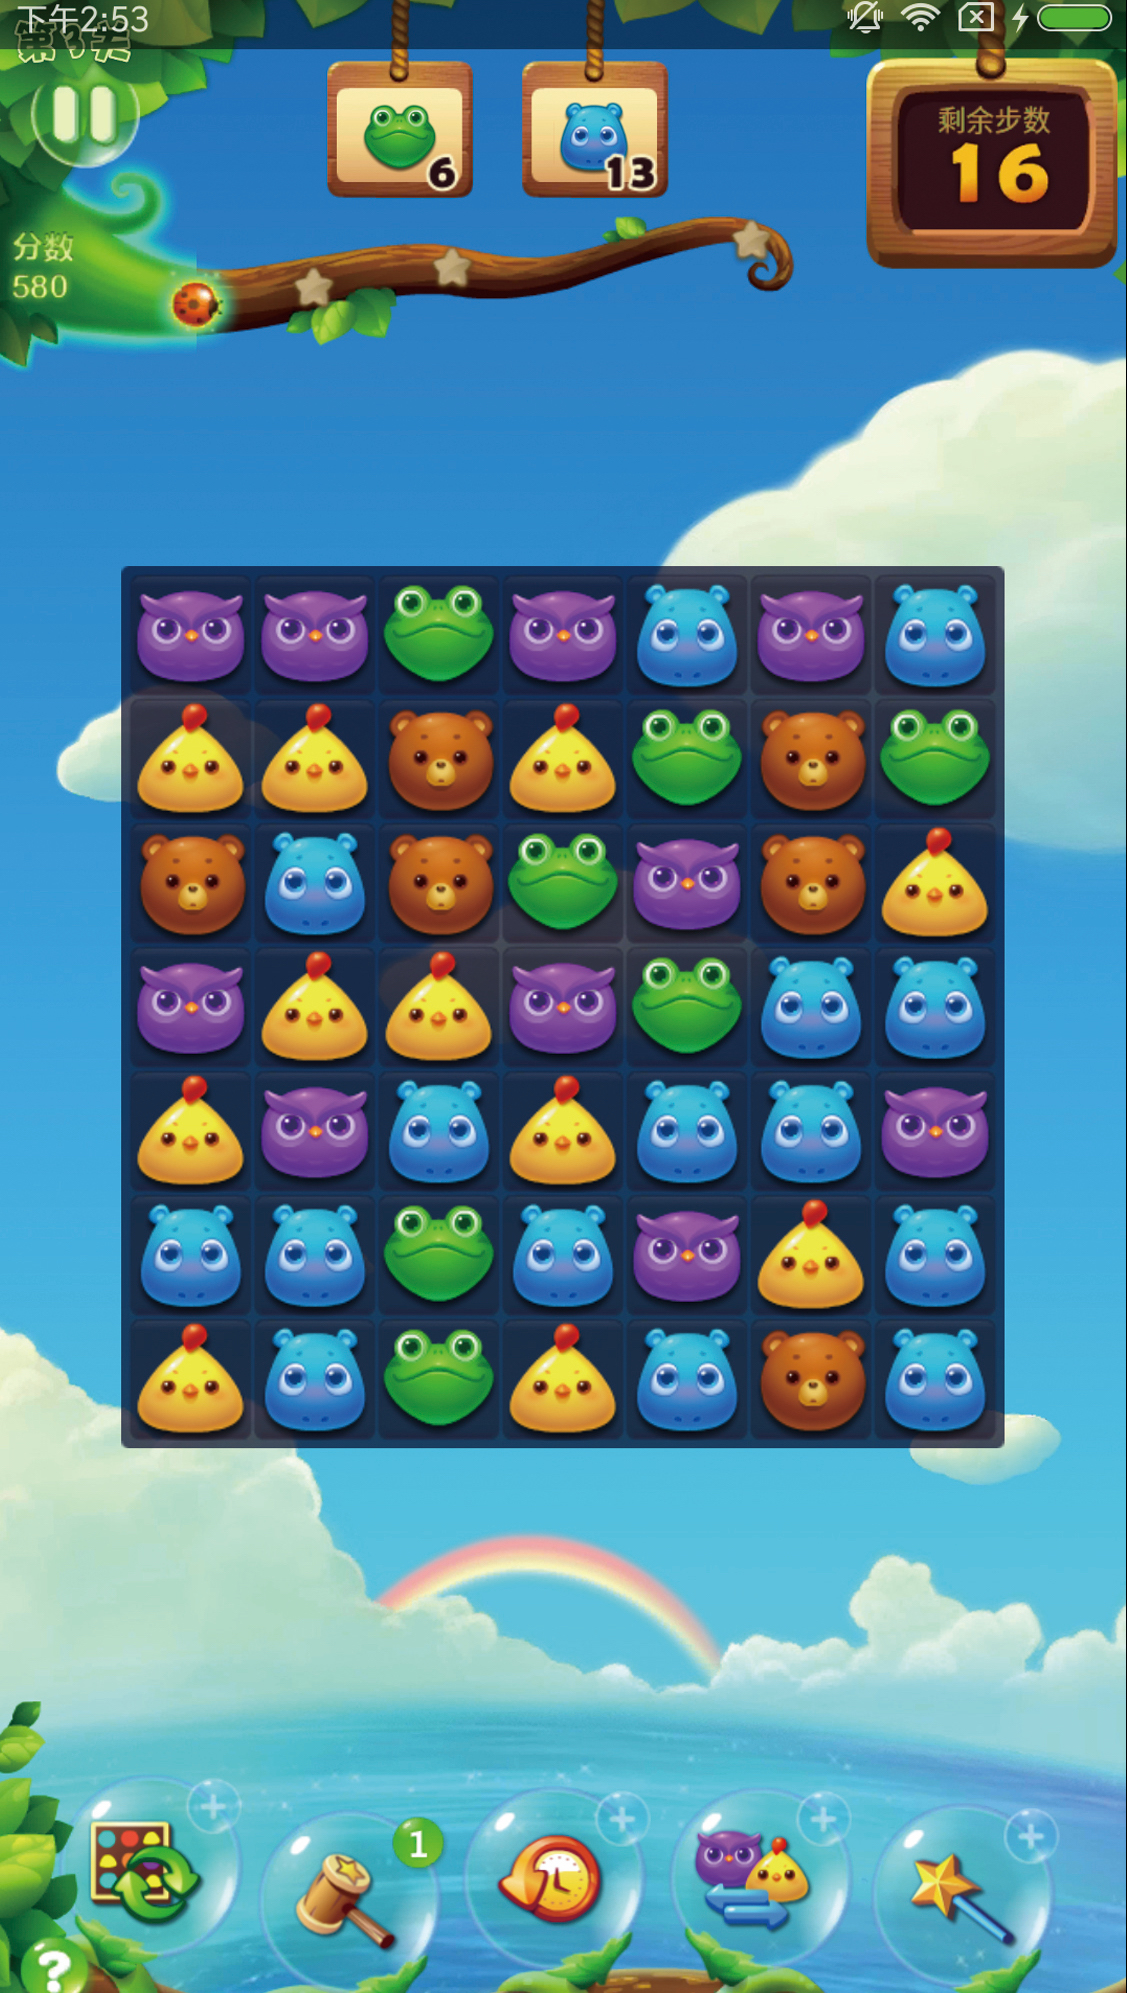
\includegraphics[width=0.3\textwidth]{./Figures/edwin-screenshot2.jpg}}\hfill
    \subfloat[仿冒版\textit{\small 开心消消乐}\label{fig:screenshot_fake}]{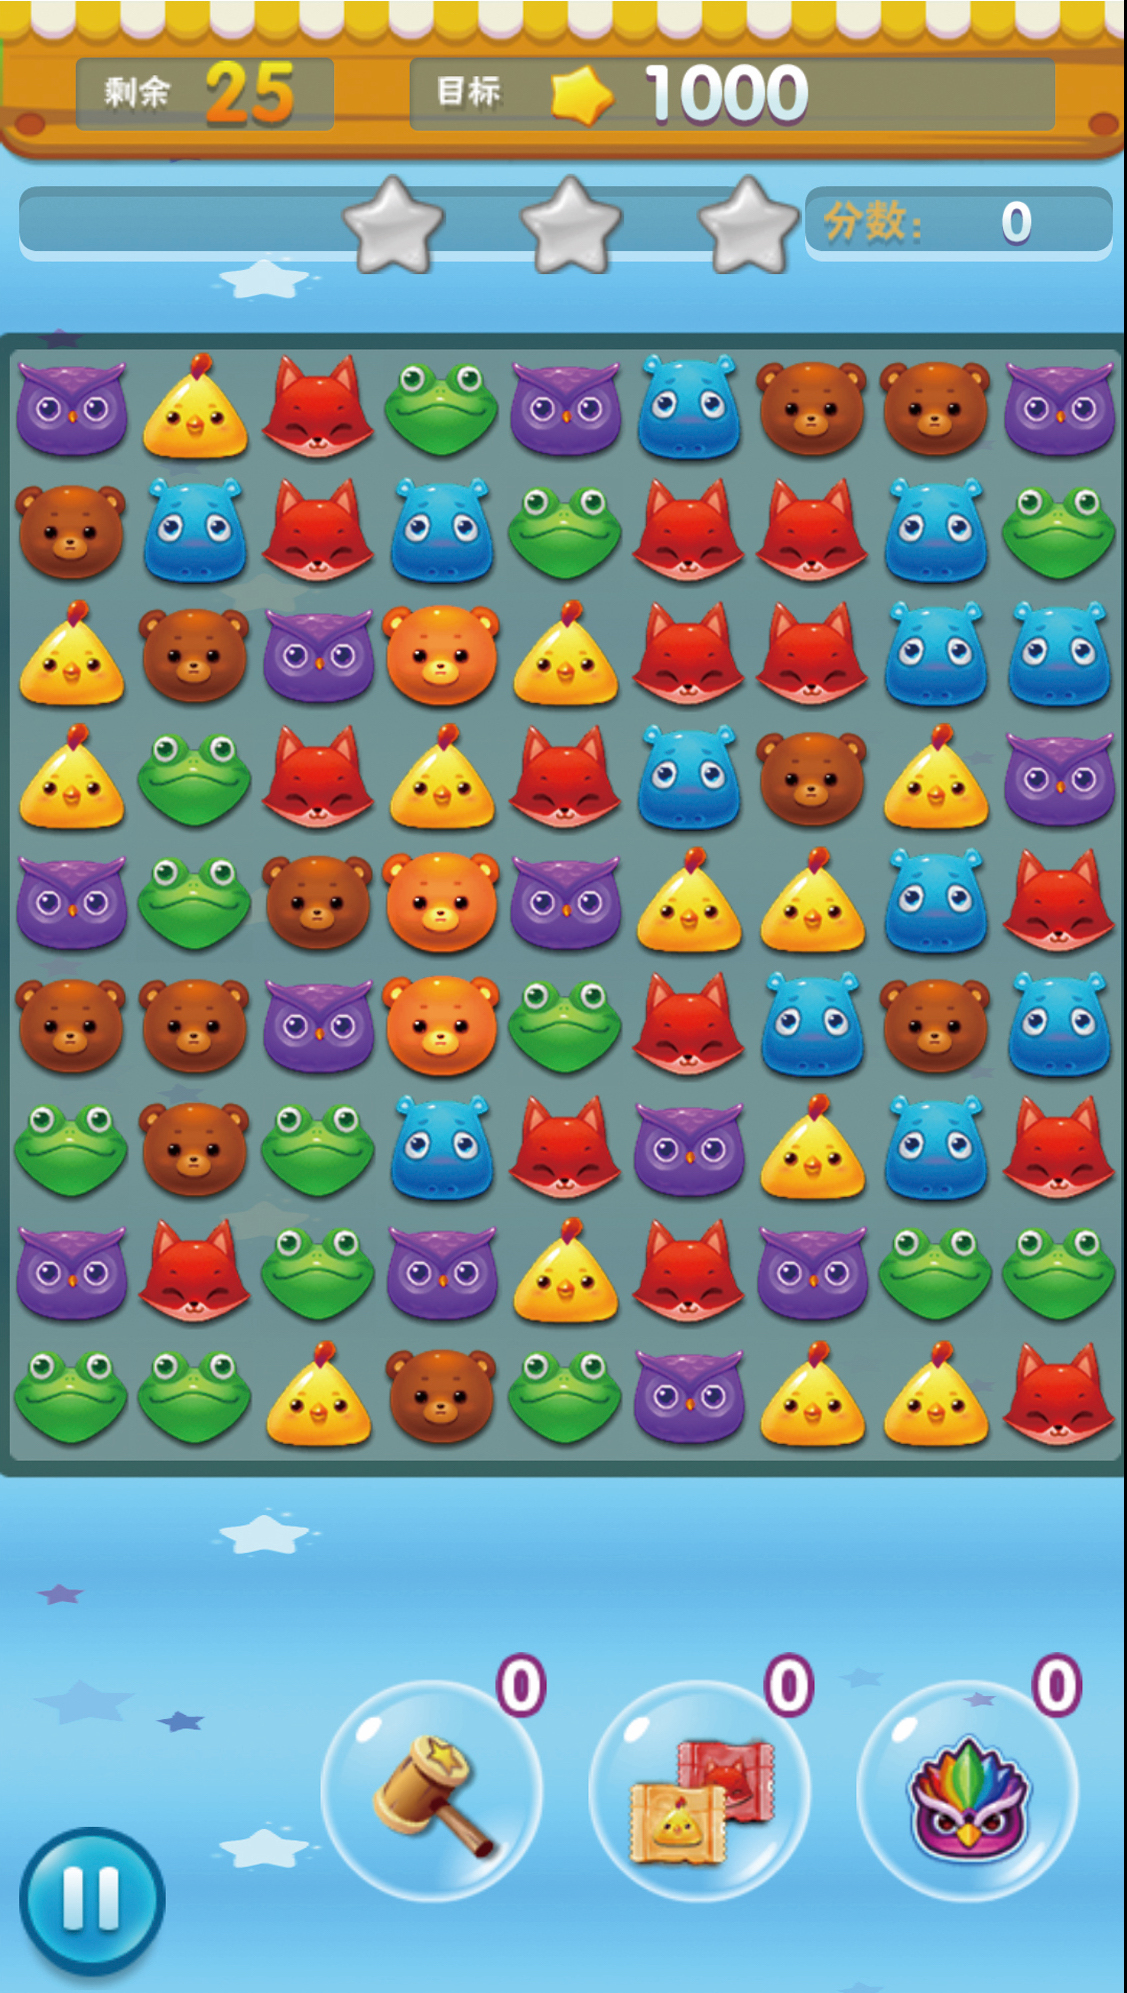
\includegraphics[width=0.3\textwidth]{./Figures/edwin-screenshot3.jpg}}\hfill
    \caption{游戏类App及其仿冒样本}
\end{figure}

% We even ran these apps on our device.
笔者在测试设备上实际运行了上述安装的14个仿冒样本,然后拿它们和原版的应用对比。
笔者使用的测试设备为高配版小米5手机,搭载的CPU为最高主频2.15GHz的骁龙820处理器,3GB内存,64GB机身存储,安装的Android系统版本为Android 6.0(Android Marshmallow,API 23)。

% Screenshots were captured when we ran one of the fake samples (see Fig.~\ref{fig:screenshot_fake}) and the official sample (Fig.~\ref{fig:screenshot_official}).
\autoref{fig:screenshot_official}和\autoref{fig:screenshot_fake}分别是在测试设备上运行官方版本的\texttt{开心消消乐}和其中一个仿冒版的\texttt{开心消消乐}时的系统截屏。
不难看出,两款应用的外观是十分相像的。
笔者在测试时发现,两款游戏内部的玩法、实际操作逻辑也一模一样。
如果不是事先知道了哪一款应用是来自官方渠道下载的正版,连笔者都没有办法判别两个应用的真伪,更不必说是从应用市场搜索结果中找到这些结果的普通用户了。

% As a result, we found that 4 fake samples of \texttt{\small HappyElements} are actually games that are similar to the official one (one is a repackaged app with high confidence), 2 are raiders on the game and the last one crashed when it was launched.
而这并不是唯一的案例。作为结果,笔者发现7款\texttt{开心消消乐}的仿冒样本中,有4款是与官方样本十分相似的游戏(其中一个十分可能是经过重打包技术处理的应用),2款声称自己是``系统攻略'',还有1款在运行时闪退,无法在测试设备上实际运行。
% 3 out of the 4 fake games pop up alert windows in the game to require users for In-App purchase, which is very possible to cause unwilling cost.
在4款仿冒游戏中,3款都在游戏中不时自动弹出游戏内购窗口,要求玩家购买道具,十分可能导致玩家不想要的花费。
% All 7 samples are reported to be malicious on \textsc{Virustotal}~\cite{virustotal}.
而所有7个仿冒样本都在\textsc{Virustotal}~\cite{virustotal}中被报告为恶意应用。

% Fake samples on \texttt{\small ArenaofValor}, in contrast, barely have functionalities like the official one.
相比之下,\texttt{王者荣耀}的仿冒样本内容就与官方应用大相径庭了。
% 3 of those samples are wallpaper setters and the rest 4 are simply puzzle games.
在7款被安装到测试设备的仿冒样本中,有3款是壁纸浏览器,里面包含了几张游戏内人物的插画,可以在应用内将这些插画设置成系统的桌面壁纸;
而余下四个是简单的拼图游戏,里面同样包含了王者荣耀游戏人物的插画,应用内容就是简单地把被打乱的插画拼图恢复原状。
% Virustotal reports 6 out of the 7 samples as malware, the last one is claimed as potentially unwanted program (PUP).
Virustotal的结果显示,7款仿冒样本中,有6款是恶意软件,涵盖了木马病毒、广告软件等类型,而余下的一款则被报告为潜在有害程序(Potentially Unwanted Program,简称PUP)。
PUP通常在用户不知情或者不愿意的情况下,通过静默安装或者捆绑安装的形式被安装在系统中。
尽管这种软件不一定包含恶意代码,但其动机十分可疑。

% We determine it is the difficulty to imitate the official app's functionality that brings about this phenomenon.
笔者认为,这种现象是由模仿正版应用功能的难易程度带来的。
% The core implementation of multiplayer online battle arena (MOBA) games like \texttt{\small ArenaofValor} is much more complicated than that in \texttt{\small HappyElements}.
只从技术角度看,像\texttt{王者荣耀}这样的多人在线战斗竞技场(Multiplayer Online Battle Arena,简称MOBA)游戏核心难度明显要比\texttt{开心消消乐}这样的益智类游戏要高得多。
一款MOBA游戏除了要解决支持运行运行的物理引擎之外,还要实现聊天系统、在线匹配、负载均衡等业务,更加不必说背后的人物设计技能平衡等更深入的话题了;而一款益智类三三消游戏的核心逻辑就只在于元素三连的判定和随机新出现的元素,再加上道具系统就差不多可以包装成一个完整的游戏推出。

% What it costs to develop a complex game like \texttt{\small ArenaofValor} is exorbitant for a fake developer.
因此,就算不考虑后续的维护问题,要开发一款像\texttt{王者荣耀}这样的复杂游戏,对仿冒应用开发者来说明显是成本过高的。
但由于这款游戏本身具有超高的热度,可能带来巨大的收益,所以仿冒应用开发者会为了蹭上热度而开发外观相似、内容完全不符的仿冒样本。
相比之下,\texttt{开心消消乐}由于开发难度相对较小,所以仿冒应用开发者会愿意开发一个内容相似的应用,再通过内购陷阱等手段收取效益。
这两款App透露出了仿冒应用开发者在仿冒方面两个截然不同的思路。

% Therefore, we can infer another reason why apps in \texttt{\small productivity} category gain a low fake sample rate:
本文在\secref{sec:quantitativeStudy}中观察到的\texttt{商务办公}类别有较低仿冒率也可能是类似原因导致的结果。
% Unlike games, on one hand, productivity tools are less likely to have peripheral products (like wallpaper setter mentioned above);
一方面,\texttt{商务办公}类的工具核心逻辑比较复杂,对仿冒开发者来说并不是一个有利可图的最佳选项;
% On the other hand, the inevitably laborious developing procedure also prevents the tools themselves from being shammed.
另外,这类应用也不像\texttt{游戏}一样会衍生出周边产品(比如\texttt{王者荣耀}的游戏人物就会有不少插画),仿冒应用开发者也没办法从这方面入手蹭热度。
结合两个原因,\texttt{商务办公}类的应用自然不会引起仿冒应用开发者的太多兴趣。

\vspace{5mm}
\noindent\fbox{
	\parbox{0.95\linewidth}{
		% \textbf{Remark 2}: As revealed by statistics, the number of samples returned from an app store does not imply a fake rate.
        \textbf{本节小结}: 正如由本文的统计和计算揭示的那样,从一个应用市场中能找到的应用样本数量并不能与应用商店的仿冒率相对应。
		% Additionally, the relationship between apps and market itself influences the number of fake samples from that market.
        此外,App本身与应用市场的关系也会影响到市场中对应App仿冒样本的数量。
		% To our surprise, an app's update frequency is not tightly correlated with its fake rate.
        出人意料的是,App的更新频率并没有与仿冒率相关联。
		% We owe this to the fact that apps are updated too frequently and that repackaged samples are of minority in our dataset.
        笔者认为这是由于应用更新频率太高、而且重打包应用在本研究的数据集中占少数而导致的结果。
		% We further observe that ``category'' as a factor has greater influence on the number of fake samples of an app than ``popularity'' and ``update frequency''.
        本文进一步观测到,与\texttt{更新频率}和\texttt{应用热度}相比,\texttt{应用分类}这一因素对App的仿冒率有更大的影响。
        案例分析从游戏类别的仿冒应用入手,说明了仿冒应用开发者对不同应用会采用不同仿冒策略。
	}
}

% \subsection{Developing Trend}
\section{仿冒应用的发展轨迹}
% In order to figure out fake apps' characteristics or behavior patterns over time, we propose the following research questions:
在这个视角下,本文希望结合时间维度,从本研究的数据中挖掘信息。
随着时间推移,仿冒应用的特征和行为模式是否有发生改变?
这些年来,仿冒应用这个灰色产业是否有过变迁?
利用本研究提取的数据中的\emph{搜集时间}数据项,本文复原了各种不同的时间线以解答上述问题。

\subsection{仿冒应用的研发延迟}
在正版应用推出新版后,如果一个仿冒应用能在越短时间内推出对应的新版本,仿冒应用的开发者就越有可能蹭上软件更新的热度,从而获利。
对此,本节提出了以下研究问题:

% \noindent{\bf RQ 3.1} After a new version of an official app is published, how long do fake developers take to publish a new fake sample? In other words, how soon will these copycats appear?
{\bf RQ 3.1}:在一个官方应用的新版本推出之后,仿冒应用开发者需要花多少时间去推出对应版本的仿冒版?
换句话说,这些``山寨''版本会过多久出现?

在分别复原官方应用的更新时间线和对应仿冒版本的发布时间之后,本文得到了以下结果:

% \noindent{\bf Answer to RQ 3.1.}
{\bf RQ 3.1. 结果}
% We compute this latency and show its distribution in Fig.~\autoref{fig:Fake_latency_overall_distribution}.
本文计算出了每版App被仿冒的延迟时间和延迟的分布情况,结果显示在\autoref{fig:Fake_latency_overall_distribution}中。

\begin{figure}
	\centering
	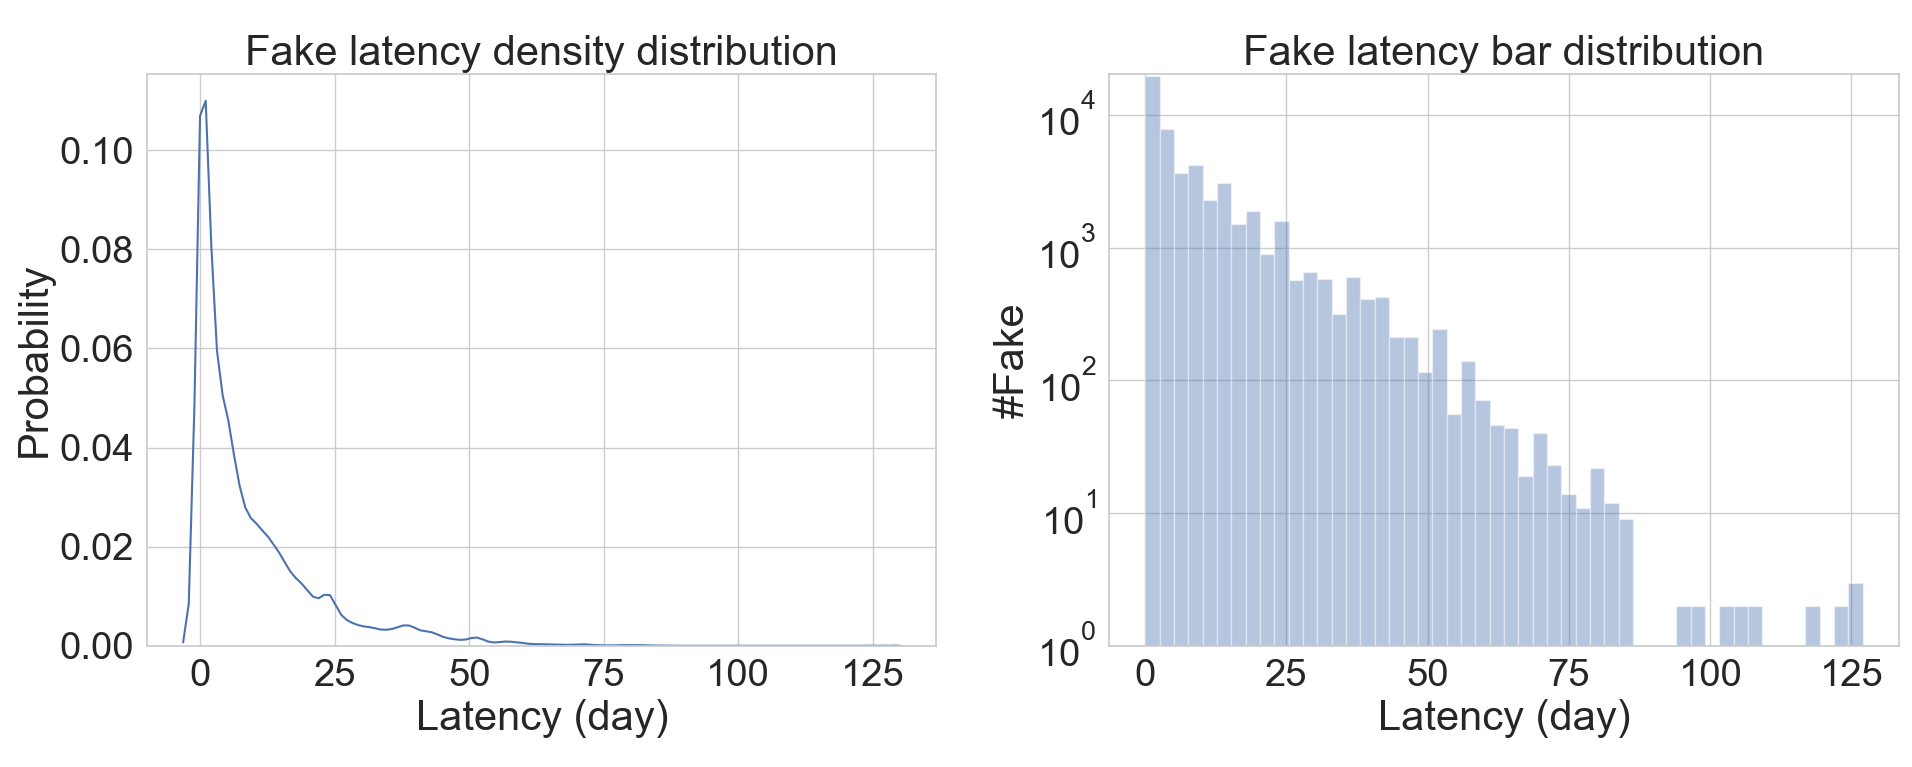
\includegraphics[width=\textwidth]{./Figures/edwin-Fake_latency_overall_distribution2.png}
	\caption{仿冒延迟总体分布}
	\label{fig:Fake_latency_overall_distribution}
\end{figure}

% Due to various reasons, it is hardly possible to retrieve the complete updating timeline for every single official app in our study, yet we approximately reproduce them with our data.
出于多种原因,本文很难为研究中的所有50款目标App回溯出它们每个版本更新的时间点,然而,凭借数据库中的数据,本文大致地重现了他们的更新时间线。
% Firstly, we categorized all the official samples by their origins, and further categorized samples in each origin by version number.
首先,本文对所有收集到的官方样本按照他们的App源进行分类,然后再按照版本号对App源类下的所有样本分类。
举个例子,一开始是使用``爱奇艺''作为搜索源的所有官方样本都会被归回``爱奇艺''类下,然后再按版本号分类。
这么做的原因是,即使是官方渠道发布的版本,有些App在不同应用市场上架的时间和内容也会略微有差别,可能会导致一个版本的正版App有多个样本的结果。
这个做法就是为了消除上述情况带来的影响。
% After that, for each app and each version the samples are sorted by the date they were crawled, so by extracting the crawled date of the first sample in each version, we can obtain the earliest date a version is released.
之后,对于每款App的每个版本,本文都按照对应样本被爬取到的日期时间戳对其进行排序。
这样的话,通过提取每个版本中第一个版本被爬取的时间,就可以知道这个版本的官方App最早的发布日期了。
% Lastly, by combining and sorting the release dates of different versions according to different apps, we can reproduce the updating timelines of our target apps.
最后,将每款App中每个版本最早的发布日期串联起来,就可以大致重现每款App的更新时间线。

% To find out the release latency of a fake app, all the dates on the timeline of the corresponding official app are compared in order to find out the smallest negative difference which we define as the release latency.
由于仿冒样本大多不是重打包应用,本研究没办法为每个仿冒样本精确匹配一个对应的正版版本,为了找到某个仿冒样本的仿冒延迟,本文提取出它被爬取的日期时间戳,然后将这个时间戳与正版更新时间线上的所有版本进行对比,找到不晚于这个仿冒样本发布的最晚发布官方版本的发行时间,然后取他们的时间差作为仿冒延迟。
% Fig.~\autoref{fig:Fake_latency_overall_distribution} shows that most fake samples are published with the latency shorter than 20 days.
按照\autoref{fig:Fake_latency_overall_distribution}的结果,绝大多数仿冒样本在官方应用推出后的20天内就被发布了。
% According to our statistics, 60\% of fake samples show up in 6 days after a new version of the official app is published.
根据本文的统计,有60\%仿冒应用在正版App被推出的6天内就被发布出来了。
% This reveals a truth that fake developers are swift in action.
这表明仿冒开发者的行动十分迅速。

\subsection{仿冒应用安全证书的存活时长}
从某个角度看,仿冒应用安全证书的存活时长反映了应用市场的监管力度大小,也能反映市场之间在安全方面是否具有良好的合作机制。
所以本节有研究问题如下:

% \noindent{\bf RQ 3.2} How long can a fake app's certificate survive?
{\bf RQ 3.2}:一个仿冒应用开发者的安全证书可以存活多久?

本文整理了不同仿冒应用安全证书的出现时间,得出了下面的结果:

% \noindent{\bf Answer to RQ 3.2.} Fig.~\autoref{fig:Fake_certificate_survival_distribution} shows the distribution of the time a fake certificate can survive in markets.
{\bf RQ 3.2. 结果}\autoref{fig:Fake_certificate_survival_distribution}展示了不同仿冒应用安全证书在应用市场里存活时间的总体分布。
% In the left density distribution subplot, $x$-axes is the latency and $y$-axes shows the probability density of data at corresponding $x$ value.
在左边的密度分布函数图中,$x$轴表示其存活的时长,$y$轴则表示了与$x$轴上的值对应的概率密度。
% The total area under the curve is 1, and the area under two $y$ values $y1$ and $y2$ is the probability of their corresponding value $x1$ and $x2$ account for in data.
曲线下的总面积为1,任意两个$y$值$y_1$、$y_2$之间的曲线下面积是其对应的$x$轴上的值$x_1$、$x_2$在数据中占有的概率。
% For example, in Fig.~\autoref{fig:Fake_certificate_survival_distribution}, the area beneath curve between 0 to 200 on $x$-axes is close to 0.8, which means nearly 80\% of certificates only survive for no more than 200 days.
比如说,\autoref{fig:Fake_certificate_survival_distribution}中$x$轴从0到200之间的值对应的$y$轴曲线下方的区域面积接近0.8,意味着约80\%的仿冒应用安全证书不会存活多于200天。

% To judge how long a fake certificate can survive is similar to how we calculate the update frequency of an app, the first time and the last time a fake sample from the same certificate gets crawled are marked.
断定一个仿冒应用安全证书存活市场的方法和前述计算应用更新频率的方法稍有类似,本文把某个安全证书关联的所有样本都找出来,提取出其中最早和最晚被爬取的样本的发布日期时间戳,然后将他们的差值的绝对值当作是这个安全证书的存活时长。
% The time when a sample was crawled from a market might be different from the time when it is available in the market, but our crawler downloads new samples from different markets by days and we also use days as the unit in our measurement, so we can approximately regard this two values as the same one.
从时长上爬取到样本的日期与样本在应用市场上实际能存活的时间稍有不同,但由于Janus的爬虫工具每日都从应用市场中爬取样本,而本文并没有其他方法可以知晓某款App具体在应用市场中上架了多久,只能近似地将上述提到的时间差当作是某个安全证书能在应用市场上存活的时间。

\begin{figure}[htbp]
	\centering
	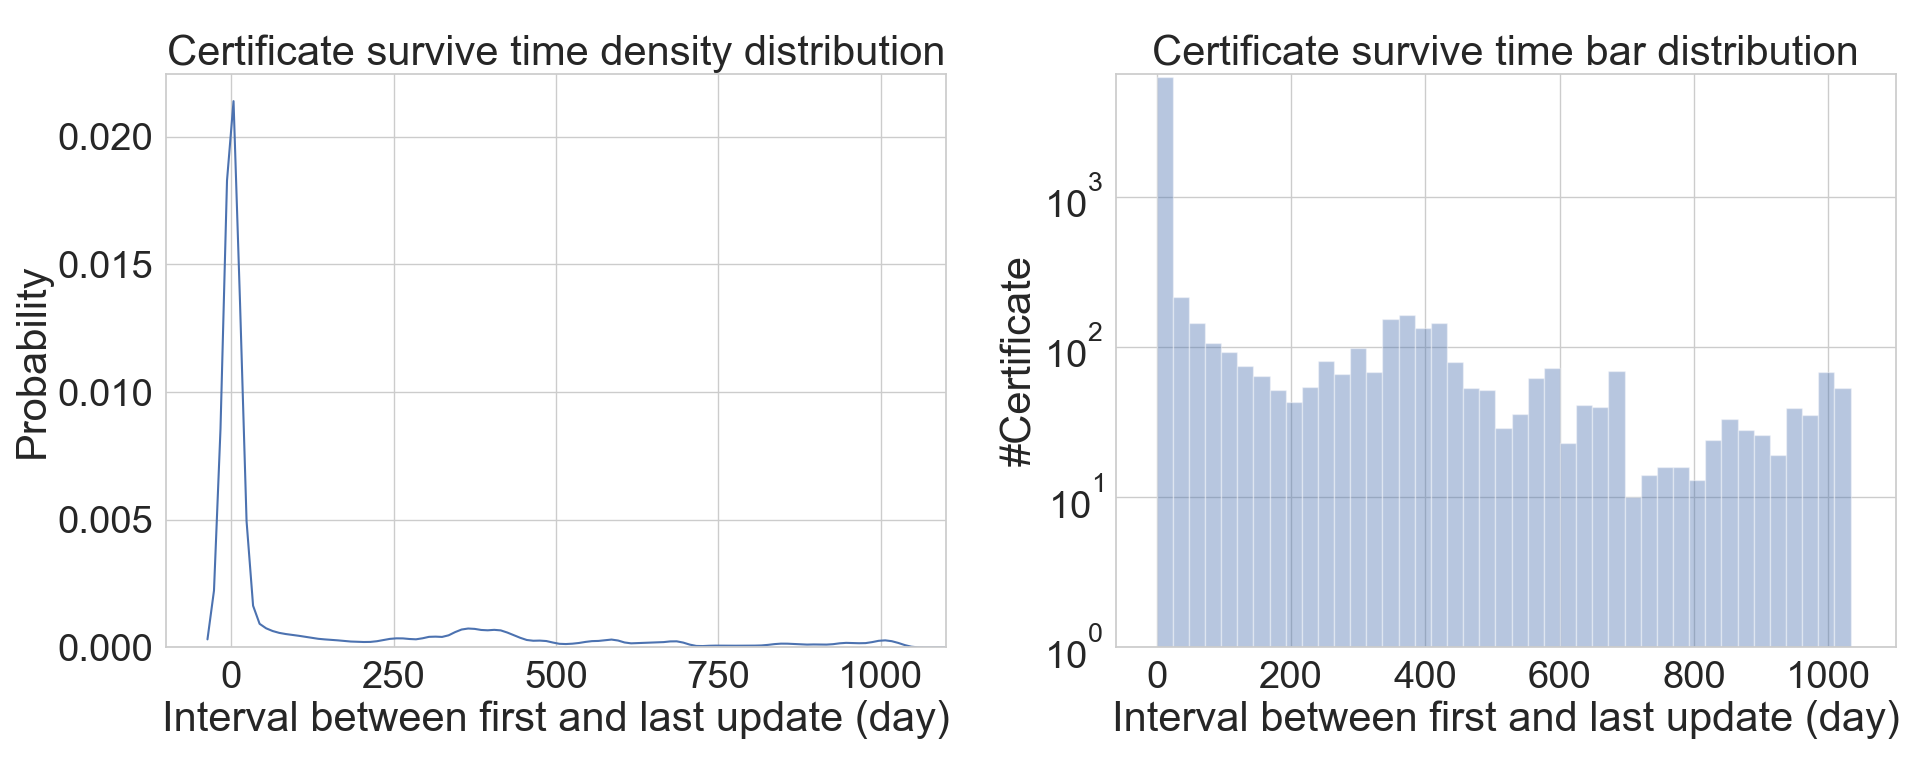
\includegraphics[width=\textwidth]{./Figures/edwin-Fake_certificate_survival_distribution2.png}
	\caption{仿冒应用安全证书存活时间分布}
	\label{fig:Fake_certificate_survival_distribution}
\end{figure}

% As shown in Fig.~\autoref{fig:Fake_certificate_survival_distribution}, the distribution of fake certificate survival time shows that almost all the fake certificates live a short life, which means most fake certificates only show up in a short period of time.
正如\autoref{fig:Fake_certificate_survival_distribution}所示,仿冒应用安全证书存活时间的分布表明几乎所有仿冒应用安全证书都只能存活相当短的时间,这表明大多仿冒应用只会在一个很小的时间窗口里出现,然后迅速消失。
% This can be explained by a scheme that most markets have.
这可以由大部分市场都有的一个安全机制解释。
% Once an app is found malicious or illegal, the market would stop that specific developer from uploading more samples by refusing to receive samples with the same certificate.
只要一款App被发现具有恶意行为或者违法行为,应用市场就会禁止开发者再使用该证书上传应用,也就是常见的封号处理。
% There are also a number of certificates which can survive for a long time.
但是,笔者也能发现有一部分的仿冒应用安全证书存活了相当久的一段时间。
% According to the figure, some fake certificates even traverse the whole study interval.
根据图表信息,可以看到有的仿冒应用安全证书的生命周期甚至贯穿了本文整个研究截取的时间周期。
% We will conduct a case study on this phenomenon in Section ~\autoref{sec:casestudy}.
对于这个异常样本,本文会在后续的案例分析中有更详尽的案例分析。

\begin{figure}[htbp]
	\centering
	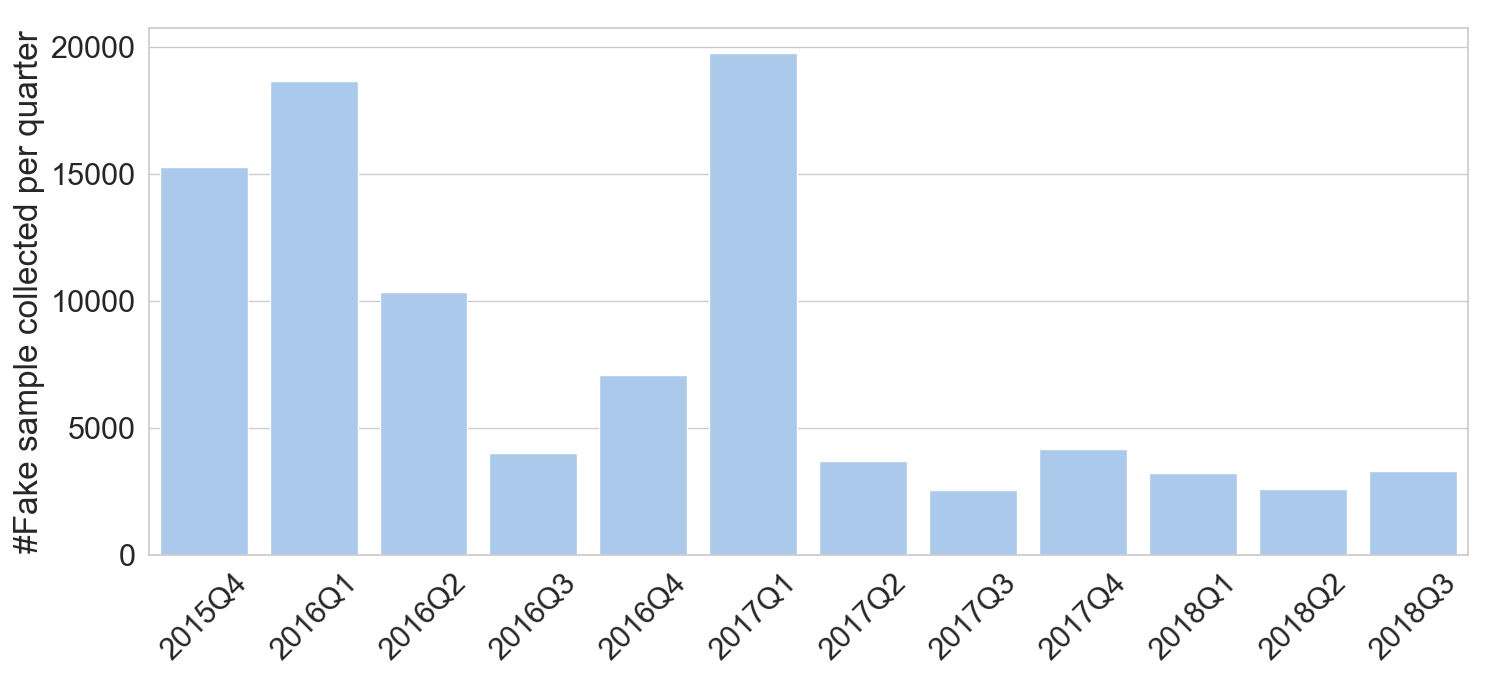
\includegraphics[width=\textwidth]{./Figures/edwin-Number_of_samples_collected_per_quarter_3.png}
	\caption{每季度爬取到的仿冒样本数量(2015年第四季度到2018年第三季度)}
	\label{fig:Number_per_quarter}
\end{figure}

\subsection{仿冒应用的行业变迁}
随着时间推移,仿冒应用这个灰色产业是否有过变迁?
本节对此提出了研究问题:

% \noindent{\bf RQ 3.3} Is there a changing pattern of fake samples over time?
{\bf RQ 3.3}:仿冒应用是否存在一个随着时间变化的模式?

笔者统计了不同时间段所搜集到的样本数量,得出了结果如下:

% \noindent{\bf Answer to RQ 3.3.} Fig.~\autoref{fig:Number_per_quarter} shows the number of fake samples collected per quarter since the fourth quarter of 2015.
{\bf RQ 3.3. 结果}\autoref{fig:Number_per_quarter}呈现了Janus自2015年第四季度起在每个季度爬取到的仿冒样本的总量。
% Although a large number of new fake samples get released in every quarter, the figure shows a tendency that the total number of fake apps on markets is gradually decreasing by years.
尽管Janus每个季度都能爬取到新上架的大量仿冒样本,图表信息表明,市场上仿冒应用的总数正在呈现逐年减少的趋势。
% Note that our statistics only focus on fake samples, consequently this phenomenon does not indicate the underground industry is turning down.
要注意的是,此处的统计仅仅针对仿冒应用。
因此这个现象并不表明移动黑灰产的发展具有萧条的趋势。
% Instead, we suppose this is possibly caused by the reform of fake apps.
相反地,本文认为这个现象更有可能是由黑灰产内部改革而导致的。

% On one hand, as stricter review schemes and stronger protection systems are applied on app stores, it's inevitable that fake apps in this study, become harder and harder to get on the shelf.
从一方面看,随着信息技术发展,应用市场逐渐配备上了更智能、严格而又强大的监管机制和安全系统,本研究中的仿冒应用开发者无疑更难以将仿冒的应用投放到市场上了。
% On the other hand, the new generation of malicious software, such as ransomware~\cite{ransomware} is impacting the underground industry.
从另一方面看,新一代的恶意软件,比如WannaCry等勒索软件~\cite{ransomware}也正在影响着整个移动黑灰产工业。
% Compare to fake apps, the new malicious apps are not only hard to defend (due to the innovative or even state-of-the-art techniques they utilize) but also extremely profitable.
与仿冒应用相比,这些新一代的恶意软件不仅更难以防范(传统的反病毒软件思路是提取已有恶意代码的特征,从而识别恶意行为,但这无法遏制新型的恶意行为),而且也似乎更容易能获取暴利。
% Wannacry, a ransomware which was first spotted in the 2nd quarter of 2017, conquered tens of thousands of devices in a couple of weeks, which directly pulled up Bitcoin's price like a rocket~\cite{wannacry_bitcoin_news}.
Wannacry作为一种新型恶意软件,自2017年第二季度被首次发现开始,就能在数周内攻克数以千万计的设备,并让比特币的价格像搭火箭一样直线飙升~\cite{wannacry_bitcoin_news}。
% Afterward, in the first quarter of 2018, a burst of cryptomining malware on phones emerged~\cite{comodo_report}.
之后不久,在2018年的第一季度,移动设备上也爆发了一系列的加密采矿恶意软件~\cite{comodo_report}。
% This may be the reason why the number of fake samples suffers two suddenly drops in the second quarter of 2017 and the first quarter of 2018, respectively.
所以笔者有理由猜测2017年第二季度和2018年第一季度的仿冒应用上架数量下跌是受到了新形态黑灰产的冲击。
当然,证实这个猜想还需要采集更多数据、进行更深入的研究。

\subsection{案例 3. 与大量仿冒应用相关联的仿冒应用安全证书}
\label{sec:case1}

% We manually review the samples signed by the certificate with SHA1 ``\emph{61ed377e85d386a8dfee6b864bd85b0bfaa5af81}", the certificate with the most number of fake samples among our fake certificate set (i.e., 1,374 fake samples).
\secref{sec:fakeCharacteristics}提到有部分仿冒应用安全证书关联着多个仿冒样本。
其中,一个SHA1码为``\emph{61ed377e85d386a8dfee6b864bd85b0bfaa5af81}''的安全证书是所有证书中关联仿冒样本最多的,足足有1,374个样本持有这个仿冒证书。
% On top of that, this certificate is also one of the certificates survive the longest time (nearly 3 years) and is still active.
不仅如此,这个安全证书还是其中一个在应用市场中存活时间最长的仿冒应用安全证书。
它的出现横穿了本研究的整个研究时间过程(接近三年),而且在本研究的数据收集流程结束前依然呈现活跃状态。

% Originally, we presume this certificate to belong to a benign app which passes the verification of analysts in Pwnzen, since the number of samples it links to even exceeds the number of official samples of some apps.
最初,笔者假定这个证书属于某个通过犇众分析团队验证的良性应用,因为它关联的样本数量实在是太大了,这个数量甚至超过了本研究中某些目标App的样本总量。
% The truth is, however, after manually review, we found all the 1,374 samples linked with this certificate are typical fake samples, in form of either imitators or imposters, covering 79\% (37 out of 47) of our target apps.
然而在人工审核之后,笔者却发现了意料之外的结果。
这个证书关联的所有1,374个样本都是典型的仿冒样本,其中既有只与原版应用稍微近似的\texttt{模仿应用},也有外观上完全模仿原版应用的\texttt{高仿应用},覆盖了本研究能找到的47个目标App中的37个(79\%)。
% Some of its samples can even be organized in version order, which means the developer does track official apps to update its fake versions as maintenance.
而这些证书关联的一些样本,甚至有自己的版本顺序,这表明有的开发者真的会追踪官方App的各个版本来更新、甚至维护自己的仿冒版本。

\begin{table}[htbp]
    \renewcommand{\arraystretch}{1}
    \small
    \centering
    \caption{由``61ed377e85d386a8dfee6b864bd85b0bfaa5af81"签署的部分样本}
    \vspace{1mm}
    \rowcolors{2}{gray!15}{white}
    \begin{tabular}{l l c c c c c c}
        \toprule
        {\bf Name} & {\bf Package Name} & {\bf Size} \\
        \midrule
        QQ Talk  & net.in1.smart.qq & 465.8 KB \\
        QQ  & com.h & 8.2 MB \\
        爱微信  & com.lovewechat & 368.4 KB \\
        微信  & com.tencen1.mm & 22.1 MB \\
        UC Mini  & com.uc.browser.en & 2.1 MB \\
        UC 浏览器  & com.UCMobile.microsoft & 21.3 MB \\
        Clean Master  & com.blueflash.kingscleanmaster & 972.0 KB \\
        WiFi万能钥匙  & com.snda.wifilocating & 5.9 MB \\
        \bottomrule
    \end{tabular}
    \label{table:certificate_case_study}
\end{table}

% We display some of the samples singed by this certificate in Table~\ref{table:certificate_case_study}, they are all reported to be malicious (i.e., Ad-ware, spyware or Trojan) on \textsc{Virustotal}~\cite{virustotal}, a famous online antivirus engine.
本文在\autoref{table:certificate_case_study}中展现了由这个安全证书签署的部分样本。
笔者将这些样本上传到知名在线反病毒引擎\textsc{Virustotal}~\cite{virustotal}上,结果显示,与该证书关联的所有样本都是恶意样本(广告软件、间谍软件或木马软件等)。
% So far the samples related to our target apps have already been showing up in 20 markets including the leading ones like \texttt{\small Myapp} and \texttt{\small Qihoo 360 Market}.
到目前为止,由这个证书签署的仿冒样本已经在本研究的20个应用来源(即应用市场)中出现,包括\texttt{应用宝}和\texttt{360应用市场}等主流应用市场。
% What's more, \texttt{\small Baidu App Store} keeps receiving apps with this certificate from 2015 to recently -- its latest ``product'' was put on shelf on September 15$^{th}$, 2018.
除此之外,\texttt{百度手机助手}从2015年起就开始接受由这个安全证书签署的应用,直到本研究的数据收集阶段结束前——数据显示,这个安全证书在2018年9月15日还在\texttt{百度手机助手}上架了一款应用。

% To this end, we can draw the following conclusions:
在这里,可以得到以下两个结论:
\begin{itemize}
    % (1) Even the leading app markets (and the top developers) are unqualified in detecting malicious apps.
    \item 就算是领先的应用市场(和顶尖的开发者)在检测恶意应用方面也不能做到尽善尽美,而现有的检测方法也有所不足,未能及时地找出可疑的开发者;
    % (2) Existing app markets lack information exchange on defending attacks from underground industry.
    \item 从这个证书在多个市场都存在的现象,笔者推导,现有的应用市场缺乏有效的信息交换机制。
    如果各个应用市场能建立一个互通信息的平台,分享可疑开发者/恶意开发者信息,那么将可以杜绝一部分恶意开发者在各个应用市场上到处流窜的现象。
\end{itemize}

\vspace{5mm}
\noindent\fbox{
	\parbox{0.95\linewidth}{
		% \textbf{Remark 3}: Fake apps can be produced in a relatively short time, and the dropping number of fake samples by years suggests that they are mired in recession.
        \textbf{本节小结}:仿冒应用可以在极短时间内被研发并上架,而仿冒样本逐年下降的新增量,也许表明了仿冒应用产业正在陷入衰退期,但这需要更多证据和研究证实。
		% Besides, only a few fake certificates survive for a long time, confirming that markets' protection schemes do work to some extent.
        此外,只有很小一部分的仿冒应用安全证书可以存活很长的一段时间,这表明应用市场的保护监管机制在一定程度上的确能发挥作用,但案例数据同时表明,现有检测方法仍有不足。
        另外,案例提供的数据也表示了应用市场之间缺乏交流恶意开发者/可疑开发者信息的平台。
	}
}

\section{本章小结}
本章先分别从\emph{仿冒应用的基本特征}、\emph{影响仿冒应用数量的因素}和\emph{仿冒应用的发展轨迹}三个不同视角对采集到的数据进行了分析,并在每个视角后的本节小结中概括了每个视角的结论,解读仿冒应用的特征。
然后,本章从数据集中选出了一些较有代表性又或者反直觉的数据样本,提供了3个不同的案例分析,在为本文的发现提供有力支持之外,也揭示了更多仿冒应用开发者的行为,深化了对仿冒应用生态的了解。

回看三个案例,不难发现,仿冒应用开发者的确会抓住一切可能的机会,利用包括签名机制漏洞、市场审查机制缺陷在内的各种办法制作出仿冒甚至是恶意应用。
同时,本章的三个案例也说明了无论是开发人员还是应用市场,都应该在保护Android的软件安全方面上投入更大精力,从而更好地防范来自移动黑灰产的各种攻击。
